\documentclass[a4paper, 12pt]{report}
\usepackage{hyperref}
\usepackage{gensymb}
\usepackage{ amssymb }
\usepackage[utf8]{inputenc} % выбор кодировки кода
\usepackage[T2A]{fontenc} % выбор внутренней кодировки 
\usepackage[english, russian]{babel} % выбор языка
% \righthyphenmin = 2 % минимальное число букв после переноса: может пригодиться
\usepackage{multirow}
\usepackage{fontawesome}
\usepackage{easyReview}
\usepackage{tabularx}
\usepackage{rotating}
\usepackage{amsmath} % русский текст в формулах
\usepackage{color} % цвет текста
\usepackage{ulem} % для зачёркивания текстаё

\usepackage[left=15mm, right=10mm, top=20mm, bottom=20mm]{geometry} % поля
\usepackage{indentfirst} % отступ первого абзаца
\setlength{\parindent}{1,25cm} % длина отступа первой строки абзаца
\linespread{1,5} % междустрочный интервал

\usepackage{titlesec} % настройка заголовков
\renewcommand{\thesection}{\arabic{section}} % противотараканная мера для report'а: делаю section заголовком первого уровня
\titleformat{\section}{\centering \large \bfseries}{\thesection}{1ex}{\MakeUppercase}{}
\titleformat{\subsection}{\centering \large \bfseries}{\thesubsection}{1ex}{}{}
\titleformat{\subparagraph}[runin]{\bfseries}{\thesubparagraph}{}{}{}

% \titleformat{\bibliography}{\centering \large \bfseries}{\thebibliography}{}{}{} % попытка настроить заголовок для списка литературы

\usepackage{graphicx}
\graphicspath{{./Photos/}}


\usepackage{comment} % Для многострочных комментариев
\usepackage{xcolor} % Для девочек 
\usepackage{enumitem}

\usepackage[
natbib		= true,
style		= gost-numeric,
sorting		= none,
backend		= biber,
language	= autobib,
bibstyle	= gost-numeric,
citestyle	= gost-numeric,
autolang	= other]{biblatex}
\addbibresource{Gvandra2024_biblio.bib}

\begin{document}
\begin{titlepage}

	\begin{center}
		РОО <<Федерация спортивного туризма Московской области>>\\
		ОО г. Долгопрудного <<Федерация спортивного туризма>>\\
	\end{center}

	
	
	\begin{center}
		\Large{\bfseries{ОТЧЁТ}} \\
		\normalsize о прохождении горного спортивного туристического маршрута первой категории сложности по Западному Кавказу (Гвандра), совершённом с 18 по 30 августа 2024 г. группой туристов Горной секции МФТИ ФСТ Московской области, г. Долгопрудный
	\end{center}
	\vspace{1.8 cm}
	
	\parskip \textbf{Маршрутная книжка:} 03.03.01, прикладные математика и физика \\ 
	\textbf{Направленность подготовки:} Физическая и квантовая электроника
	\vspace{3 cm}
	
	\null\hfill
	\begin{minipage}{0.5\textwidth}
		\begin{flushleft} \large
			\textbf{Студент:} \\
			Остапив Алексей Юрьевич
			\vspace{0.5 cm}
			\hrule
			\vspace{-0.6 em}
			\begin{center}
				\small \textit{(подпись студента)} \\
			\end{center}
			
			\vspace{-0.4 em}
			\large
			\textbf{Научный руководитель:} \\
			Коняшкин Алексей Викторович \\
			к.ф.-м.н., старший научный сотрудник ФИРЭ им. В.А. Котельникова РАН 
			\vspace{0.5 cm}
			\hrule
			\vspace{-0.6 em}
			\begin{center}
				\small \textit{(подпись научного руководителя)} \\
			\end{center}
			
		\end{flushleft}
	\end{minipage}
	
	% \vspace{4.3cm}
	\vfill
	\vfill
	\begin{center}
		Москва   \the\year{}
	\end{center}
	
\end{titlepage}
\renewcommand{\contentsname}{Содержание}
\tableofcontents
\clearpage
\section*{Сокращения, используемые в отчёте}
\addcontentsline{toc}{section}{Сокращения, используемые в отчёте}
\section{Справочные сведения о походе} 
\subsection{Проводящая организация}
\subsection{Место проведения}
\subsection{Общие справочные сведения о маршруте}
\subsection{Подробная нитка маршрута}
\subsection{Определяющие препятствия маршрута}
\subsection{Список участников} 
Тут будет список наших \sout{долбанов} зайчиков.
\newpage
\section{Организация и проведение похода}
\subsection{Цели и задачи маршрута. Подготовка, выбор маршрута}
Даша, необходимо твоё творчество. 

\textcolor{teal}{Окэй. Итак...} 

При места проведения маршрута в целом, я как руководитель опиралась на следующие соображения: 
\begin{enumerate} 
	\item Транспортная доступность горного района и стоимость трансфера. 

	Поскольку группа, как я и надеялась, практически полностью состояла из новичков, в этом случае особенно важно было затратить минимум сил и средств на логистику, --- т.~е. выбрать район с наилучшей транспортной доступностью за наименьшие деньги. При такой постановке задачи почти автоматически отсеиваются районы дальнего, и ближнего зарубежья --- расположенные, например, в Киргизии --- а также вся азиатская часть России, как, например, Алтай, --- и дальнейший выбор сводится фактически к одному из районов Кавказа. 
	
	\item Концентрированность препятствий 
	Дополнительным фактором в сторону выбора Кавказа послужило также и то, что в отличие, например, от Алтая, для этих гор характерны довольно короткие долины, поэтому подход к перевалам занимает, как правило, один день и позволяет поддерживать интерес группы на приемлемом уровне \textcolor{teal}{(нас это, правда, не спасло, хех)}. 
	
	\item Разнообразие рельефа  
	С методической точки зрения, а также, опять-таки, для поддержания интереса, хотелось продемонстрировать участникам как можно больше разнообразных типов рельефа: в частности, осыпной в диапазоне от крупных до мелких осыпей, и, самое главное, снег и лёд. В связи с этим 
\end{enumerate} 

\subsection{Изменение маршрута и их причины}
Маршрут пройден без изменений.
\subsection{Развёрнутый график движения}
\begin{table}[h!]
	\centering
	\resizebox{0.9\textwidth}{!}{%
	\begin{tabular}{|>{\centering\arraybackslash}m{0.045\linewidth}
								|>{\centering\arraybackslash}m{0.02\linewidth}
								|>{\centering\arraybackslash}m{0.43\linewidth}
								|>{\centering\arraybackslash}m{0.04\linewidth}
								|>{\centering\arraybackslash}m{0.07\linewidth}
								|>{\centering\arraybackslash}m{0.05\linewidth}
								|>{\centering\arraybackslash}m{0.043\linewidth}
								|>{\centering\arraybackslash}m{0.085\linewidth}|}
		\hline						
		Дата	&	\begin{turn}{90}День\end{turn}	&	Участок маршрута	&	\begin{turn}{90}Км с $k=1.2$\end{turn}	&	Набор /сброс, м	&	ЧХВ	&	\begin{turn}{90}Высота ночёвки, м\end{turn}	&	Способы передвижения	\\
		\hline
		
		18.08	&	1	&	г.~Минеральные воды~--- аул Верхний Учкулан~--- д.р Учкулан~--- д.р. Кичкинакол Уллукёльский	&	хзхз	&	$+454$\newline$-0$	& 4:88	&	2000	&	Машина,\newline Пешком	\\
		\hline
		19.08	&	2	&	д.р. Кичкинакол Уллукёльский~--- оз. Гитче-Кёль~--- оз. Уллу-Кёль 	&	7,2	& $+700$\newline$-0$		& 5:20		& 2700		&	Пешком	\\
		\hline
		20.08	&	3	&	м.н.~--- \textbf{пер. Уллу-Кёль Восточный (1А$^\star$, 3050)}~--- кош в д.р. Трёхозёрная~--- д.р. Махар	&	4	&5		&6		&7		&	Пешком	\\
		\hline
		21.08	&	4	&	м.н.~--- т/б <<Глобус>>~--- д.р. Гондарай~--- д.р. Джалпаккол	&	4	&5		&6		&7		&	Пешком	\\
		\hline
		22.08	&	5	&	м.н.~--- д.р. Кичкинекол Джалпаккольский~--- м.н. под моренным валом пер. Джалпаккол Северный	&	4	&5		&6		&7		&	Пешком	\\
		\hline
		23.08	&	6	&	м.н.~--- \textbf{пер. Джалпаккол Северный (1А$^\star$, 3411)}~--- зелёные ночёвки на спуске в д.р. Мырды	&	4	&5		&6		&7		&	Пешком	\\
		\hline
		24.08	&	7	&	м.н.~--- д.р. Мырды~--- а/л <<Узункол>>	&	4	&5		&6		&7		&	Пешком	\\
		\hline
		25.08	&	8	&	м.н.~--- д.р. Кичкинекол~--- д.р. Таллычат~--- Поляна Крокусов	&	4	&5		&6		&7		&	Пешком	\\
		\hline
		26.08	&	9	&	м.н.~--- \textbf{пер. Кичкинекол Малый (1А, 3206)}~--- д.р. Чунгур-Джар	&	4	&5		&6		&7		&	Пешком	\\
		\hline
		27.08	&	10	&	м.н.~--- \textbf{пер. Перемётный (1А, 3255)}~--- д.р. Танышхан	&	4	&5		&6		&7		&	Пешком	\\
		\hline
		28.08	&	11	&	м.н.~--- д.р. Чиринкол~--- д.р. Кубань &	4	&5		&6		&7		&	Пешком	\\
		\hline
		29.08	&	12	&	м.н.~--- погранзастава <<Хурзук>>~(рад.)~--- д.р. Уллу-Кам	&	4	&5		&6		&7		&	Пешком	\\
		\hline
		30.08	&	13	&	м.н.~--- \textbf{пер. Хотютау (1А$^\star$, 3546)}~--- лед. Большой Азау~--- оз. Эльбрусское~--- ст. <<Старый Кругозор>>~--- поляна Азау&	4	&5		&6		&7		&	Пешком, Канатная дорога	\\
		\hline
	\end{tabular}
	}

\end{table}



\newpage
\section{Литературный обзор по прохождению маршрута} % FIXME Кривая формулировка, надо заменить 

\subsection{Пер. Уллу-Кёль Восточный} 
Перевал Уллу-Кёль Восточный расположен в северо-восточном отроге Даутского хребта и связывает д.~р. Кичкинакол Уллу-Кёльский с д.~р. Махар. В самом этом разветвлении, между хребтом и отрогом, находится каскад из двух озёр: собственно оз. Уллу-Кёль (карач.-балк. <<Большое озеро>>) и оз. Гитче-Кёль (карач.-балк. <<маленькое озеро>>). Озеро Уллу-Кёль, по описаниям, исключительно живописно и является значимой достопримечательностью района --- однако единственный доступный для походов 1 к.~с. выход из цирка, в котором оно располагается, --- это пер. Уллу-Кёль Восточный, который с технической точки зрения был самым сложным среди всех перевалов нашего маршрута, и который, по идее, нельзя рекомендовать в качестве первого. 

Альтернативой перевалу Уллу-Кёль Восточный может служить пер. Уллу-Кёль Нижний (н/к), через который в д.~р. Махар можно попасть от нижнего озера, Гитче-Кёль, --- именно этим маршрутом прошёл в 2018 г. Андрей Королёв, и именно этот вариант был знаком руководителю. Замена однако при этом получается совершенно неравнозначной: с одной стороны, Уллу-Кёль Нижний идеально выполняет функцию акклиматизационного перевала, а с другой стороны, при проходе через него теряется возможность увидеть верхнее озеро, Уллу-Кёль, --- если только не идти на него радиально. В связи с этим, при планировании маршрута вставал вопрос о том, стоит ли рассматривать маршрут через оз. Уллу-Кёль и пер. Уллу-Кёль Восточный, или же следует удовлетвориться видом оз. Гитче-Кёль и пройти через Уллу-Кёль Нижний. В конечном итоге руководитель пошёл на риск и проложил маршрут через Уллу-Кёль Восточный, назначив вариант через Уллу-Кёль Нижний запасным: существенную роль в этом сыграло нежелание полностью копировать машрут Королёва, а также сильная нелюбовь руководителя к радиальным выходам. 

Перевал ориентирован с ССЗ на ЮЮВ. На перевальном взлёте со стороны озера большую часть времени лежит снег, сам взлёт в верхней своей части достигает крутизны 40--50\degree~и заканчивается снежным карнизом. Вероятность, что группа в итоге пойдёт на этот перевал, руководителем оценивалась примерно в 30\%; ставку при этом планировалось делать: 1) на благоприятную ориентацию склона со стороны подъёма; 2) на то, что во второй половине августа снега будет меньше, чем это фиксировалось в среднем в отчётах; 3) на то, что все участники группы будут оснащены кошками. 
\subsection{Джалпаккол Северный} 
Перевал Джалпаккол Северный должен был представлять из себя второй по сложности перевал на маршруте после Уллу-Кёля Восточного. Руководитель проходил этот перевал в 2018 году, и в том походе, по отзывам участников, с точки зрения он был явно лидирующем. Характерной особенностью перевала является наличие под его взлётом ледовой линзы, которую приходится огибать, проходя под гребнем из разрушенных скал. Этот участок камнеопасен, и в нём заключается первая опасность при прохождении данного перевала. Вторая опасность заключается в том, что есть возможность сорваться и укатиться на несколько десятков метров вниз по ледовой линзе: в 2018 году руководитель стал свиделем этого. Особенно велика вероятность этого при прохождении перевала без кошек, поэтому, как уже было сказано выше, от участников кошки требовались в обязательном порядке. Наконец, третья ключевая особенность перевала --- пятиметровый участок разрушенных скал перед выходом на седловину, который приходится преодолевать свободным лазанием. Для некоторых участников, которые неуверенно себя чувствую на скалах, этот участок мог стать большой проблемой. 

Перевал ориентирован с северо-запада на юго-восток, что несколько смягчает условия его прохождения с точки зрения раскисания снега и камнеопасности, однако по-прежнему рассматривался руководителем как один из самых сложных. Альтернативой данному перевалу мог бы служить Джалпаккол Южный (1А), расположенный, соответственно, южнее, но поскольку Джалпаккол Северный, с одной стороны, разнообразнее и богаче с точки зрения техники, а с другой стороны, у руководителя был опыт его прохождения, то выбор был сделан однозначно в его пользу. 

При прохождении перевала группа опиралась на воспоминания руководителя и отчёт Королёва Андрея \cite{Korolyov2018}, а также на отчёты...
\subsection{Кичкинекол Малый} 
Перевал Кичкинекол Малый расположен  в северном отроге ГКХ, отходящем от вершины Кичкинеколбаши к югу от вершины 40 Лет Татарии, связывает д.~р. Кичкинекол и Чунгур-Джар и ориентирован с ССЗ на ЮЮВ. Проходился руководителем в 2018 году. С технической точки зрения, это самый простой перевал на маршруте и один из самых живописных: при прохождении его со стороны Кичкинекола оптимальным местом ночёвки является т.~н. Поляна крокусов --- пересохшее озеро с проходящим через него руч. Таллычат. При впадении в озеро ручей проходит через бараньи лбы, образуя водопад высотой 10--20 м буквально на расстоянии вытянутой руки от места ночёвки. Также, насколько можно судить, поляна, ручей и окрестный луг облюбованы горными козлами, и в этом месте велик шанс их встретить \cite{Korolyov2018}. При составлении маршрута, когда нужно было сделать выбор между двумя перевалами: пер. Кичкинекол Малый и конкурирующего с ним пер. Доломиты Южный, расположенного севернее в этом же хребте, --- выбор был сделан в пользу Кичкинекола Малого именно благодаря его живописности. При прохождении планировалось опираться, традиционно, на воспоминания руководителя и отчёт Королёва Андрея \cite{Korolyov2018}; также в качестве источника использовался отчёт Брунарского Дмитрия \cite{Brunarsky2023}. 
\subsection{пер. Перемётный} 
Пер. Перемётный представляет из себя одно из ключевых и, с точки зрения тактики прохождения, одно из самых сложных препятствий на маршруте. На сайте Вестры \cite{WestraCat} имеется всего пять упоминаний об этом перевале, одно из которых — фотоальбом вершин и перевалов Кавказа \cite{caucatalogue}, и ещё одно — отчёт Королёва А.~Э. 2018 г. \cite{Korolyov2018}, в котором автор принимал участие, и в ходе которого было решено отказаться от сквозного прохождения Перемётного, заменив его радиальным. Что касается остальных трёх источников, то это отчёты Зеленцовой Е.~А. 2000 г. \cite{Zelentsova2000}, Истягиной Е.~Е. 2015 г.~\cite{istyagina2015} и Анучиной С. 2019 г. \cite{Anuchina2019}: в первых двух пер. Перемётный берётся с запада на восток, из д.~р. Чунгур-Джар в д.~р. Танышхан, а в третьем --- с востока на запад, из д.~р. Танышхан в д.~р. Чунгур-Джар. 

Основную сложность при прохождении перевала с запада на восток представляет спуск: как в отчёте Зеленцовой, так и в отчёте Истягиной, описаны сложности, с которыми сталкивается группа как при планировании спуска, так и в процессе. Обоим руководителям пришлось забирать влево по ходу движения, обходя каньон ручья и мощные скальные выходы, но даже при этом группы Зеленцовой и Истягиной попадали в ловушку из труднопроходимых зарослей рододендрона и берёзового криволесья. Впрочем, после спуска оба автора указывают на возможный оптимальный вариант спуска, который пролегает ещё левее (севернее), в обход криволесья. 

Их выводы полностью подтверждает отчёт Анучиной С. от 2019 г., которая вела группу из трёх человек по каменистому распадку --- руслу пересохшего ручья --- в обход берёзового криволесья. Судя по описанию, этот вариант выглядит довольно щадящим и представляет из себя в основном путь по курумнику с небольшим участком рододендроновых зарослей наверху и высокой травы у подножия склона. В том же отчёте утверждается, что по левому берегу р. Танышхан проходит тропа, которая сливается с тропой, ведущей по левому берегу р. Чунгур-Джар. 

Идея взять Перемётный возникла в качестве альтернативы прохождению очень неприятного участка вдоль Чунгур-Джара: крутого спуска вдоль водопада по заросшему рододендронами склону. Технически на этом склоне имеется тропа, но, по моим воспоминаниям, она легко терялась, и, в целом, склон был усеян небольшими камнями размером с ботинок, которые невозможно было разглядеть сквозь рододендроновые заросли, и на которых ничего не стоило подвернуть ногу. В случае же с Перемётным мы будем иметь тоже не самый приятный для группы, но более предсказуемый и оттого безопасный спуск по курумнику и обещанную тропу, которая проходит по травянистой долине без большого сброса. Таким образом, я решаю разменять гарантированно неприятный и небезопасный спуск на, предположительно, более долгий, но чуть более безопасный спуск; предположительно терпимую тропу и взятие нового нетривиального перевала с исследованием предположительно оптимального по нему маршрута. 
\subsection{пер. Хотютау} 
Перевал Хотютау (1А, 3550 м) расположен на Юго-Западном ребре Эльбруса, ориентирован с запада на восток и связывает долину одного из левых притоков р. Уллу-Кам (которая, в свою очередь, является правым притоком -- родоначальником Кубани) с ледовыми полями Эльбруса (нижней плоской частью лед. Большой Азау). Этот перевал также проходился руководителем в 2018 году, и, по воспоминаниям, не вызвал сложностей. На тот момент, с учётом времени года, перевальный взлёт с обеих сторон был осыпным: со стороны р. Уллу-Кам довольно занудным, но технически простым, а со стороны Эльбруса до момента выхода на ледник --- коротким и простым. Прохождение же ледовых полей Эльбруса хотя и могло сорваться в случае, если бы ледник оказался закрытым, но вероятность этого в нашем случае, во второй половине августа, была низкой. В связи с этим ориентироваться на месте предполагалось в первую очередь на воспоминания руководителя и отчёт Королёва Андрея (кон.~июля -- нач.~августа 2018) \cite{Korolyov2018} соответственно, а также на отчёты Александра Севидова (вторая половина июля 2021) \cite{Sevidov2021} и Дмитрия Брунарского (кон.~июля -- нач.~августа 2023) \cite{Brunarsky2023}.
\section{Техническое описание маршрута}
\subsection{18 августа. Старт}
\newpage
\subsection{19 августа. Д.р. Кичкинакол Уллукёльский}

Подъём дежурных в 05:00, общий подъём в 05:30 \remove{под бодрую еврейскую песню на гуслях <<Ломирр зих ибербетн>>.~ }
Выходим в 07:30, идём по 

\begin{figure}[h]
	\centering
	\includegraphics[width=0.7\linewidth]{../pics/DSC_0658}
	\caption{Группа в верховьях д.р. Кичкинакол Уллукёльский}
	\label{fig:DSC_0658}
\end{figure}

\begin{figure}[h]
	\centering
	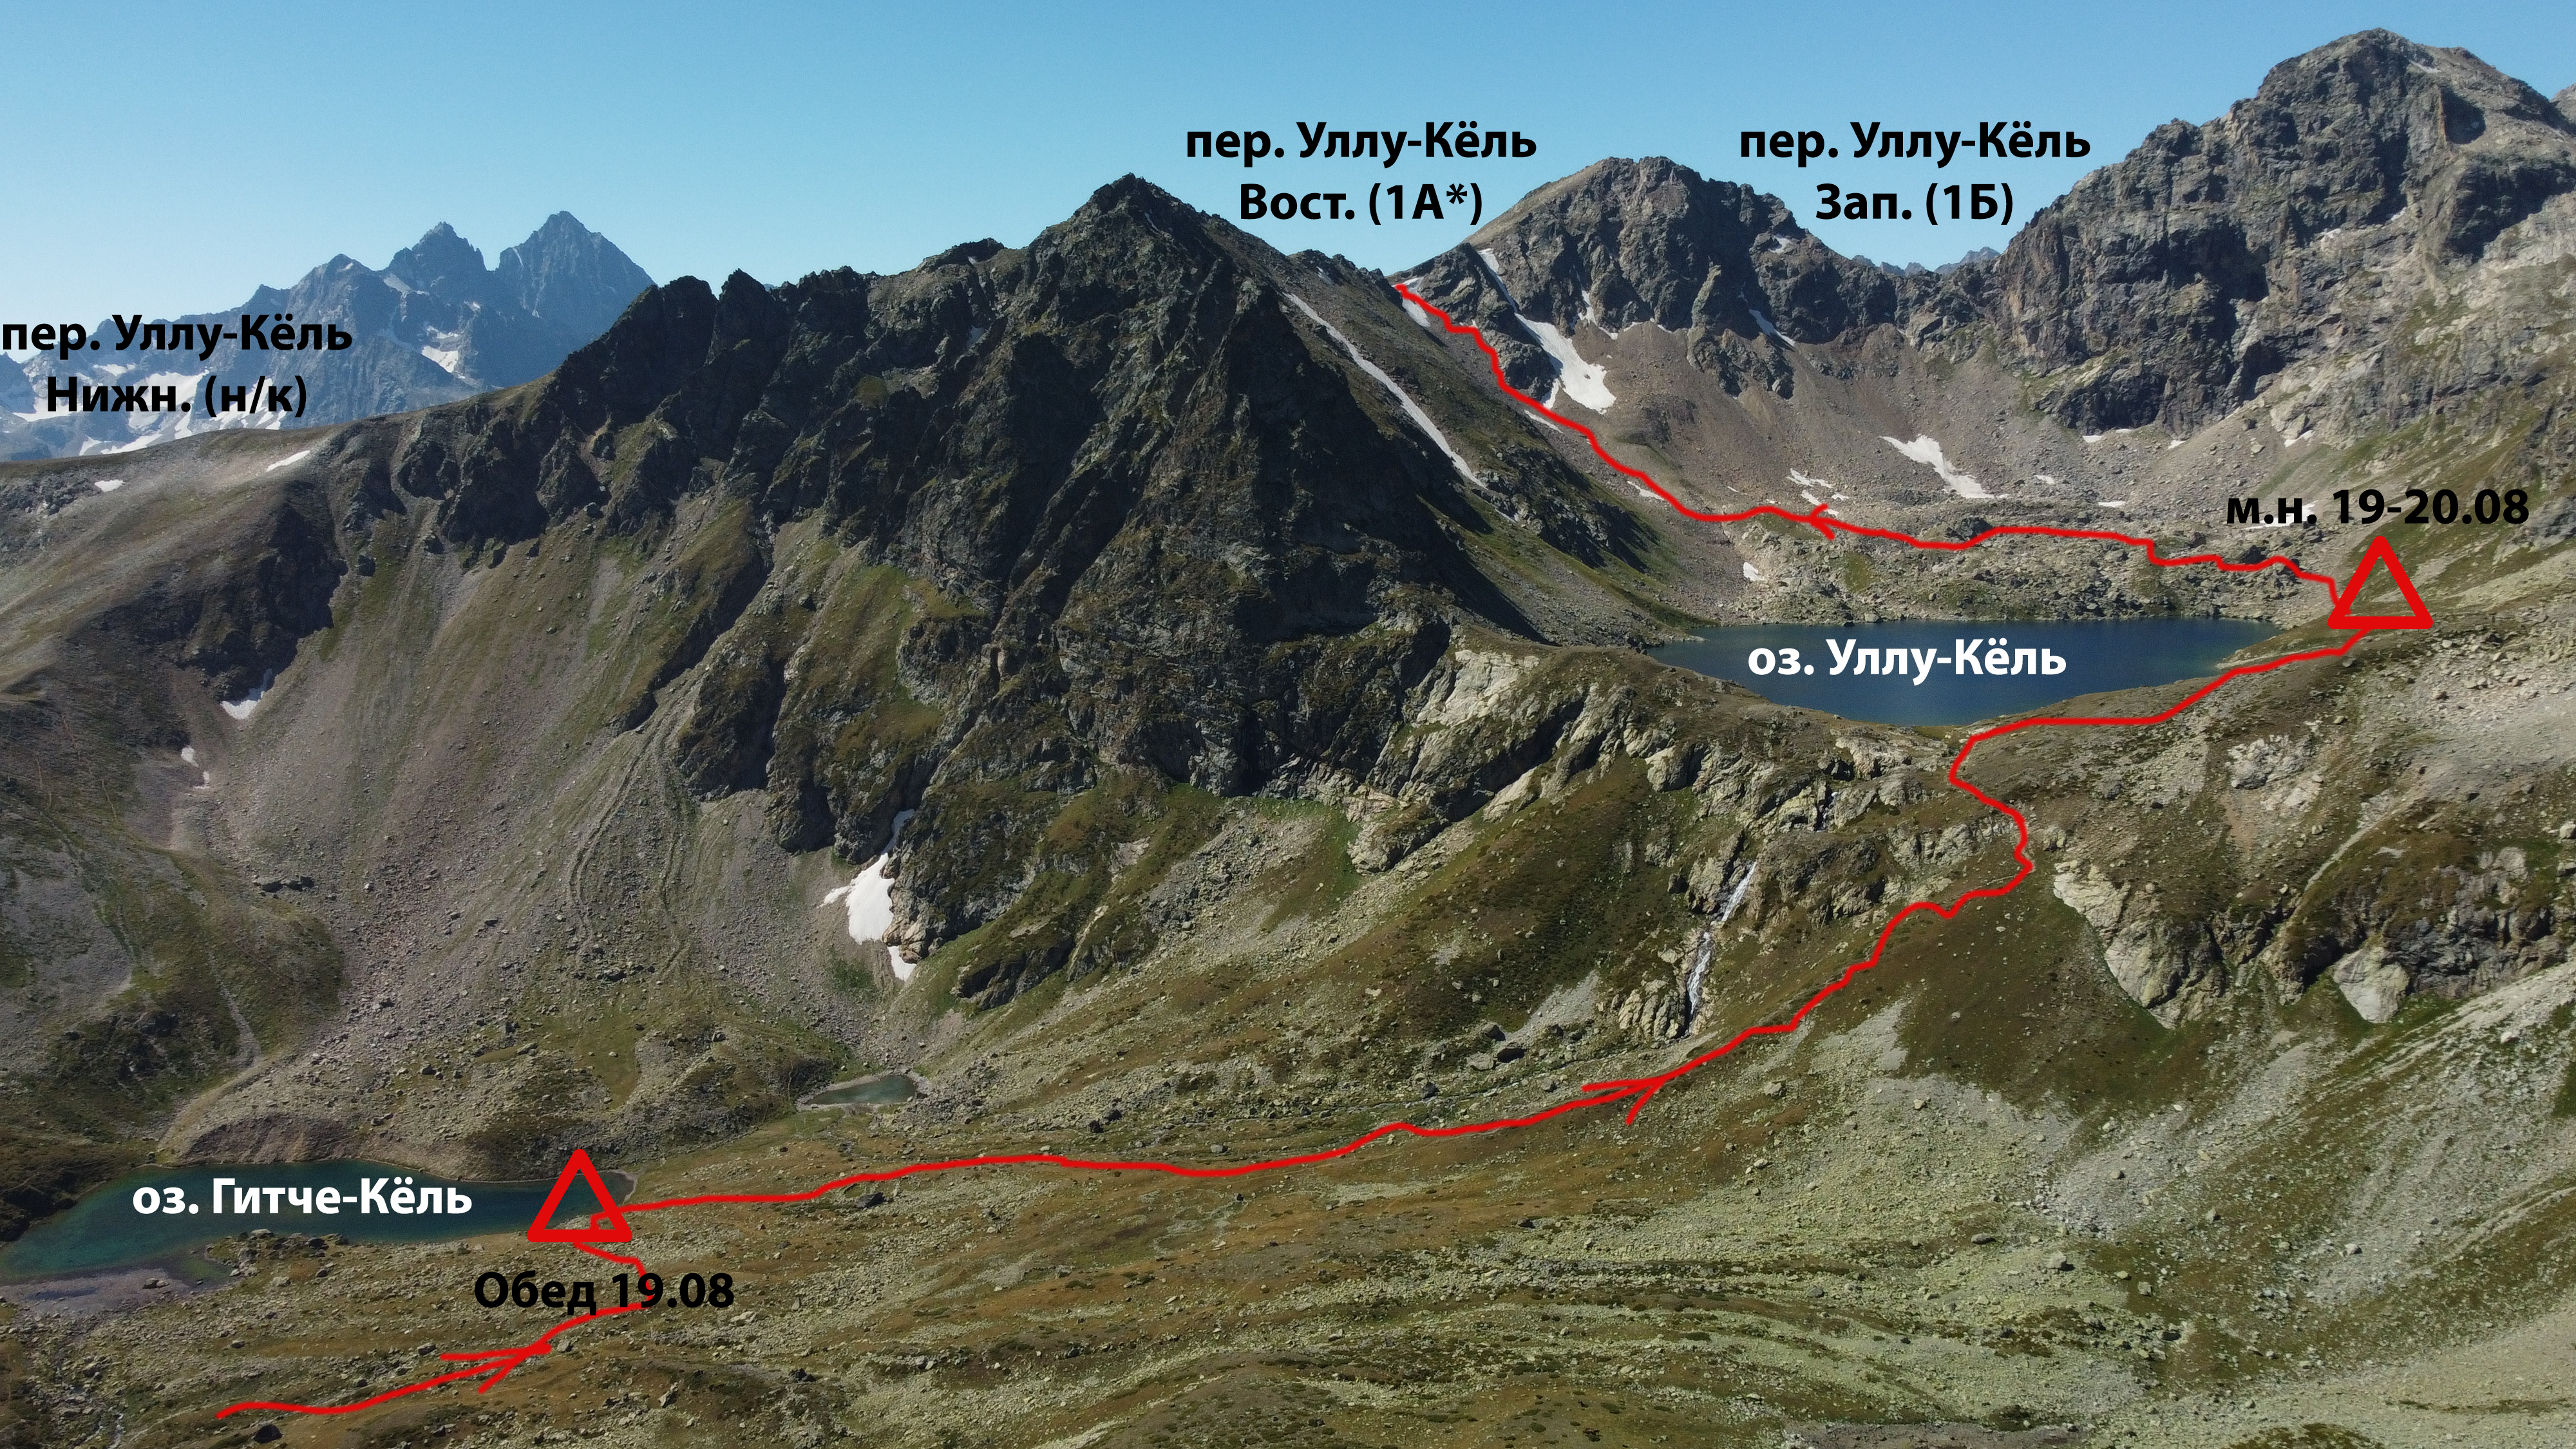
\includegraphics[width=0.7\linewidth]{../pics/ullu_kuel_route}
	\caption{Дорога до озёр и далее на перевал}
	\label{fig:ullu_kuel_route}
\end{figure}

\begin{figure}[h]
	\centering
	\begin{turn}{90}
		\includegraphics[width=0.7\linewidth]{../pics/DSC_0774}
	\end{turn}
	\caption{Купаемся в оз. Гитче-Кёль}
	\label{fig:DSC_0774}
\end{figure}

\begin{figure}[h]
	\centering
	\includegraphics[width=0.7\linewidth]{../pics/DSC_0800}
	\caption{Группа на оз. Уллу-Кёль}
	\label{fig:DSC_0800}
\end{figure}

\newpage
\subsection{20 августа. пер. Уллукёль Восточный (1А*)}
\textit{Метеоусловия: утром, днём ясно, вечером~--- переменная облачность, тепло.}

\begin{figure}[h!]
	\centering
	\includegraphics[angle=0, width=0.7\linewidth]{../pics/mini_maps/20}
	\label{fig:mini_20}
\end{figure}

Подъём дежурных в 04:30, общий подъём в 05:00. Выход группы в 07:30 (рис.~\ref{fig:20aug1.jpg}).

\begin{figure}[h!]
	\centering
	\includegraphics[width=0.7\linewidth]{../pics/20aug1.jpg}
	\caption{Подход под перевал от м.н.}
	\label{fig:20aug1.jpg}
\end{figure}


 Движемся по разведанному вчера маршруту по крупной осыпи в обход южной оконечности озера. На одном из привалов участнице (Наташе Мироновой) становится нехорошо, и часть пути (ок. 15 мин. ЧХВ) она проходит без рюкзака. Пока доносим рюкзак, группа фотографируется на фоне озера на небольшом зелёном гребешке (рис.~\ref{fig:DSC_0907}).
 
 \begin{figure}[h!]
 	\centering
 	\includegraphics[width=0.7\linewidth]{../pics/DSC_0907}
 	\caption{Фоткаемся на фоне озера}
 	\label{fig:DSC_0907}
 \end{figure}
 

Далее движемся на юго-восток по морене до другого зелёного гребешка, ведущего под перевальный взлёт (рис.~\ref{fig:20aug2.jpg}) и в 9:40 выходим на среднюю осыпь перевального взлёта, прижимаясь к правому пхд борту кулуара. Осыпь живая, требует внимания при движении и контроля неопытных участников.

\begin{figure}[h!]
	\centering
	\includegraphics[width=0.7\linewidth]{../pics/20aug2.jpg}
	\caption{Маршрут движения по перевальному взлёту}
	\label{fig:20aug2.jpg}
\end{figure}

Снега на перевальном взлёте почти нет, поэтому руководитель принимает решение двигаться не по линии падения воды, а по правому борту кулуара. Осыпь местами живая, движемся не спеша. В 12:25 достигаем полочки, на уровне которой начинается самая крутая часть перевального взлёта и снежник. Надеваем кошки и движемся косым траверсом влево пхд, чтобы выйти на седловину. Снег мягкий, возможно организовывать ступени, если ставить ногу на всю ступню. На седловине снежного карниза нет, но присутствует удобный снежный карман (рис.~\ref{fig:DSC_0946}). За 70 м тропёжки произвели две смены лидера.

\begin{figure}[h!]
	\centering
	\includegraphics[width=0.7\linewidth]{../pics/20aug3.jpg}
	\caption{Движение по правому пхд борту кулуара}
	\label{fig:20aug3.jpg}
\end{figure}

\begin{figure}[h!]
	\centering
	\includegraphics[width=0.7\linewidth]{../pics/20aug4.jpg}
	\caption{Вершины и перевалы цирка Уллу-Кёль}
	\label{fig:20aug4.jpg}
\end{figure}

Когда до снежного кармана (безопасной зоны) оставалось около 3 м по вертикали, лидер, (Катя), срывается. Пролетев 50 метров по снежному склону крутизной 45\degree, Катя не успевает окончательно зарубиться и останавливается только на осыпном склоне, перекувыркнушись через голову. Сразу после падения голосовыми командами убеждаемся, что пострадавшая в сознании. Катя в течение минуты проводит самостоятельный осмотр и убеждается в отсутствии сильных кровотечений. Руководитель и заместитель решают довести группу до безопасной зоны~--- снежного кармана, после чего спуститься к Кате. Последний человек покидает опасную зону спустя 7 минут после срыва, после чего Даша и Лёша спускаются к Кате, убеждаются, что она может идти самостоятельно, дают воду, еду и пуховку. Далее втроём поднимаемся к группе. Катя без рюкзака идёт посередине (рис.~\ref{fig:DSC_0946}).


\begin{figure}[h!]
	\centering
	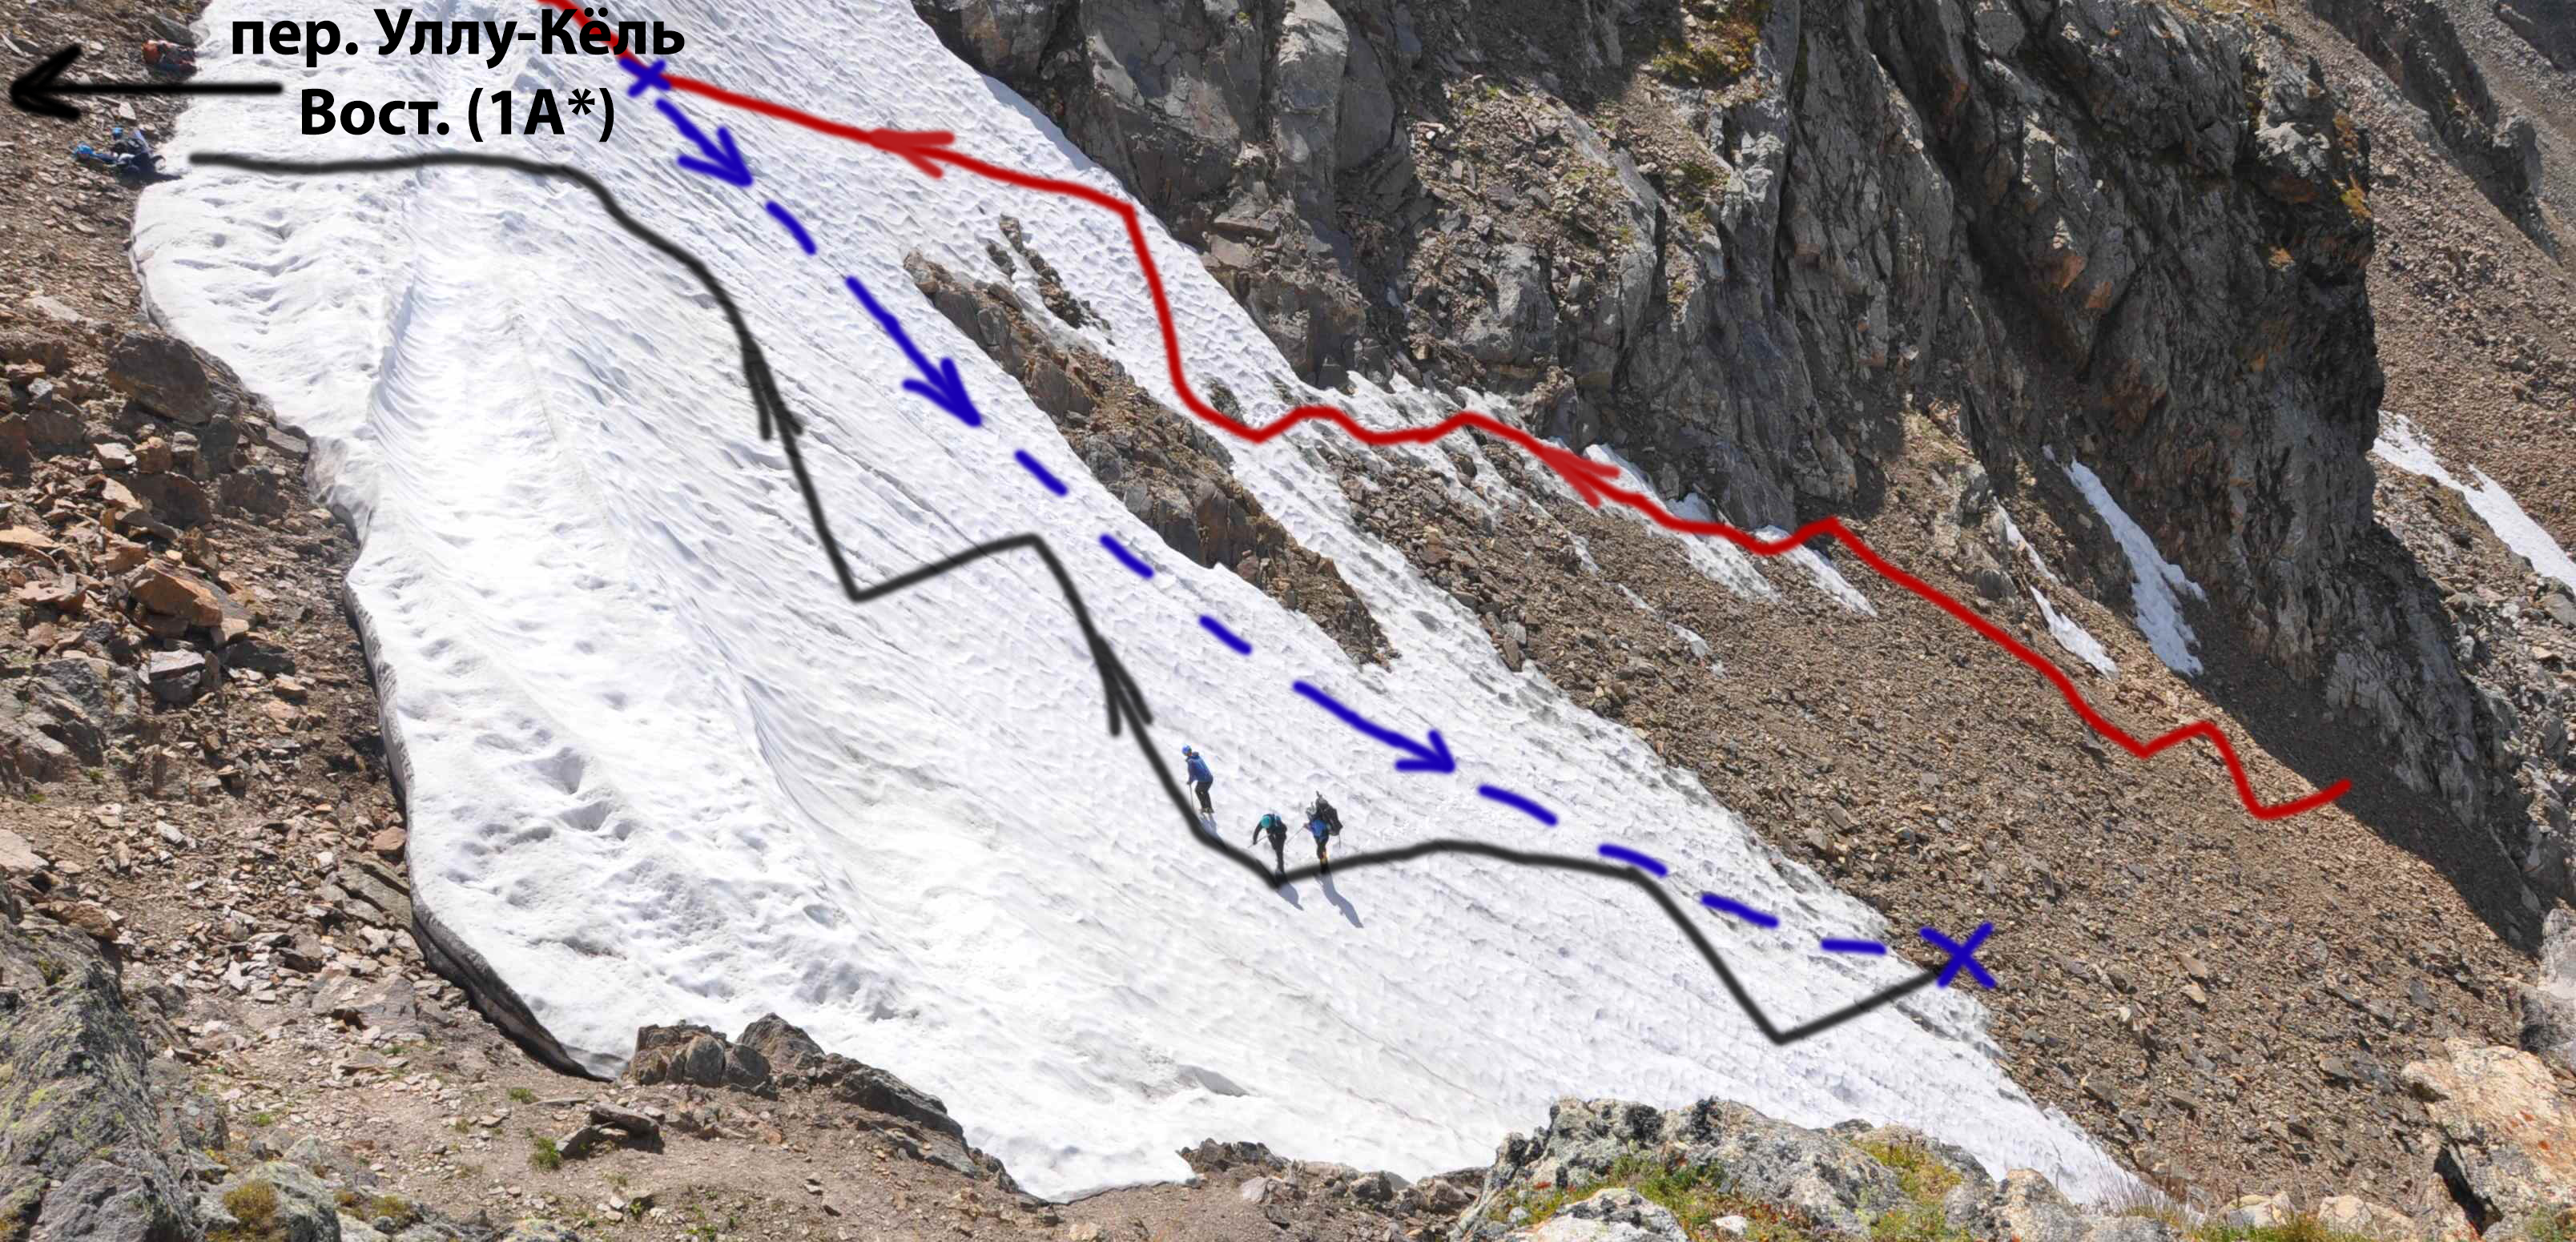
\includegraphics[width=0.7\linewidth]{../pics/DSC_0946.png}
	\caption{Маршрут движения группы по снежнику (красный), траектория срыва участника (синий), маршрут подъёма с сорвавшимся участником (чёрный)}
	\label{fig:DSC_0946}
\end{figure}

Вся группа собирается на седловине в 14:30. Снимаем записку туристов т/к <<Шторм>>, г~.Санкт-Петербург, от 09.08.2024.

\begin{figure}[h!]
	\centering
	\includegraphics[width=0.7\linewidth]{../pics/DSC_0982}
	\caption{Группа на перевале, вид на д.р. Махар}
	\label{fig:DSC_0982}
\end{figure}

\begin{figure}[h!]
	\centering
	\includegraphics[width=0.7\linewidth]{../pics/DSC_0986}
	\caption{Группа на перевале, вид на оз. Уллу-Кёль}
	\label{fig:DSC_0986}
\end{figure}


В 15:48 выходим на спуск. Катя чувствует себя хорошо и идёт со своим рюкзаком.
Спускаемся к озеру по пологому травянистому склону, далее--- по гребню.

\begin{figure}[h!]
	\centering
	\includegraphics[width=0.7\linewidth]{../pics/IMG_20240820_164917.jpg}
	\caption{Спускаемся по гребню к озеру}
	\label{fig:IMG_20240820_164917.jpg}
\end{figure}

Приходим на озеро в 16:52, устраиваем обед. В 18:10 выходим, по дороге думаем, стоит ли ночевать у коша пастухов или лучше спуститься в д.р. Махар (рис.~\ref{fig:IMG_20240820_184645.jpg}).

\begin{figure}[h!]
	\centering
	\includegraphics[width=0.7\linewidth]{../pics/IMG_20240820_184645.jpg}
	\caption{Спуск в д.р. Махар}
	\label{fig:IMG_20240820_184645.jpg}
\end{figure}

Спускаемся к кошу в 20:16. Уже темно, идём с фонариками. Узнаём у пастуха, что до долины 1.5~км по хорошей тропе, что вкупе с небольшим сбросом (300 м) сподвигает участников проголосовать за спуск в долину и ночёвку внизу. Спуск технически несложный, мешали спуску разве что пыль и мошки. Также сказывается общая усталость группы. На начальном участке тропа узкая, в момент выхода к р. Трёхозёрнаяя становится шире.

В 22:15 встали на ночёвку в д.р. Махар, координаты м.н. N43.294527\degree,~E41.956866\degree.

\clearpage 

\begin{table}[h!]
	\centering
	\begin{tabular}{|c|c|c|c|c|c|} 
		\hline 
		Этап & ЧХВ \\ 	
		\hline 
		Подъём в д.р. Кичкинакол Уллукёльский  & 02:10 \\
		Подъём по д.р. Кичкинакол Уллукёльский  & 04:23 \\
		От м/н до начала осыпного перевального взлёта & 01:33\\ 
		По перевальному взлёту до снежника & 01:22\\ 
		По снежнику до седловины (не считая срыва участника) & 00:40\\ 
		К озеру & 00:57 \\
		К кошу пастухов & 01:56 \\
		По лесу в д.р. Махар & 01:15 \\
		\hline
		\textsc{Полное время подъёма на перевал  }& 10:08\\
		\textsc{Полное время спуска с перевала }& 04:08 \\
	\textsc{	Полное время прохождения перевала }& 14:16 \\
		\hline
	\end{tabular}
	\caption{Расклад времени, пер. Уллу-Кёль Восточный}
\end{table}

\paragraph{Выводы и рекомендации:} Наш опыт подтверждает, что категория сложности перевала занижена. В малоснежный сезон снежный карниз отсутствует, однако перемещение по осыпному и снежному склонам требует определённого уроовня подготовки группы. В снежный сезон для неопытной группы провешивать перила при такой крутизне склона потребуется почти наверняка. В новичковом походе проходить Уллу-Кёль Восточный первым по счёту перевалом не рекомендуется, поскольку, хотя его прохождение и даёт возможность посмотреть на красивое озеро Уллу-Кёль, но велик риск, во-первых, излишне утомить группу, а во-вторых --- сформировать неправильное представление о характерной сложности перевалов категории 1А, а это может иметь непредсказуемые последствия. 

\clearpage

\subsection{21 августа. Т/б <<Глобус>>}

\begin{figure}[h!]
	\centering
	\includegraphics[angle=0, width=0.3\linewidth]{../pics/mini_maps/21}
	\label{fig:mini_21}
\end{figure}

\begin{figure}[h]
	\centering
	\includegraphics[width=0.7\linewidth]{../pics/DSC_1167}
	\caption{Группа пересекает р. Гондарай по мосту из бревён}
	\label{fig:hondaray}
\end{figure}
\newpage
\subsection{22 августа. Д.р. Джалпаккол}
\textit{Метеоусловия: утром, днём ясно, вечером~--- переменная облачность, тепло. Ночью сильная гроза.}

Из-за позднего завершения ходового дня накануне устраиваем подъём достаточно поздно, в 08:00, и выходим в 10:00. Движемся по правому берегу р. Джалпаккол, не переходя на левый берег у коша N 43.296700\degree,~E 42.046662\degree. Тропа хорошо наибита, место часто посещаемо: обогнали группу пенсионеров, поднимавшихся от т/б <<Глобус>> к водопадам д.р. Кичкинекол Джалпаккольский.

\begin{figure}[h!]
	\centering
	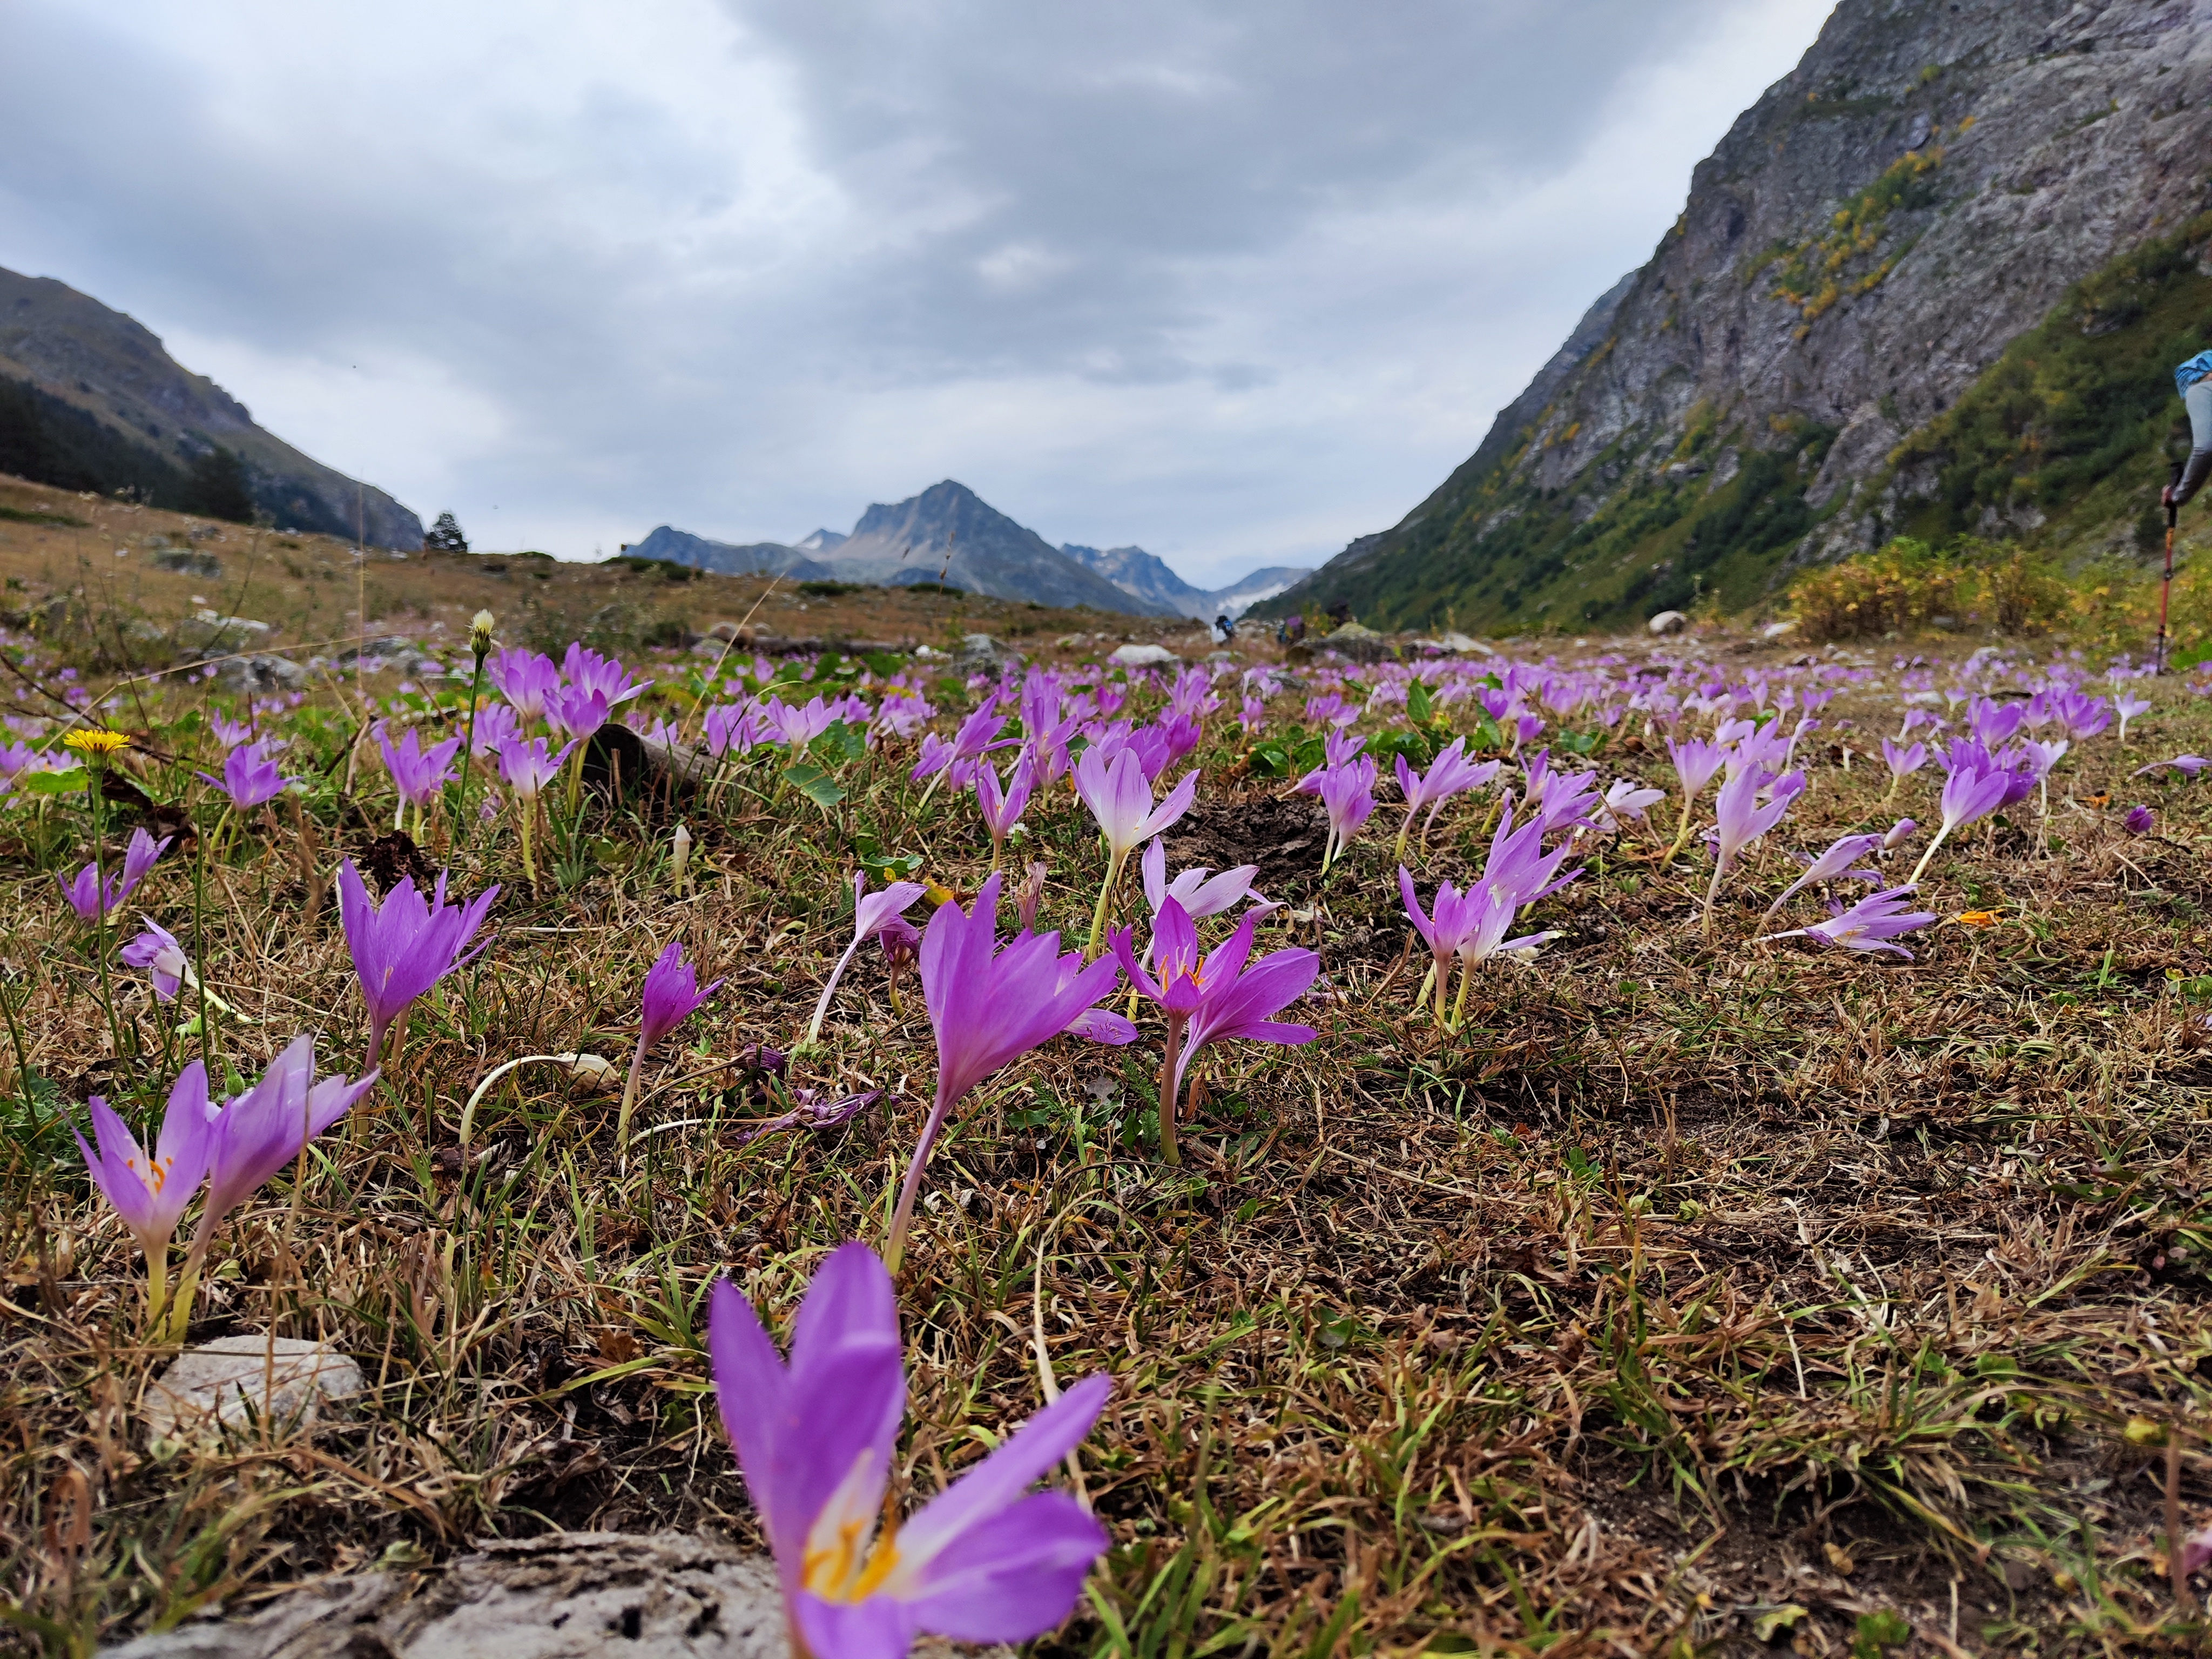
\includegraphics[width=0.7\linewidth]{../pics/IMG_20240822_101505}
	\caption{Крокусы в д.р. Джалпаккол}
	\label{fig:IMG_20240822_101505}
\end{figure}

В 11:45 дошли до развилки

\newpage
\subsection{23 августа.  Пер. Джалпаккол Северный (1А)}
\textit{Метеоусловия: утром ясно, тепло; после 16:00 туман, дождь; ночью ясно.}

\begin{figure}[h!]
	\centering
	\includegraphics[angle=0, width=0.7\linewidth]{../pics/mini_maps/23}
	\label{fig:mini_23}
\end{figure}


Подъём в 04:30, выход в 07:30. С места ночёвки на следующую ступень долины идёт довольно крутой подъём по помеченной турами тропе (рис.~\ref{fig:23augstart}); затем тропа выходит на моренные валы. Спустя 2 перехода участница Наташа Миронова сообщила руководителю о том, что у неё начались проблемы с коленями и высказала опасения, что пройти поход до конца она не сможет. \alert{(Уточнить у Кати время и симптомы.)} В 08:50 мы оказались на развилке троп (левая пхд тропа вела на каскадные озёра). Встретили семейную пару туристов с собакой, которые спускались с перевала через эти озёра. Там же сделали привал, на котором Наташе сделали противоотёчное тейпирование и выдали компрессионный наколенник.

\begin{figure}[h!]
	\centering
	\includegraphics[angle=0, width=0.7\linewidth]{../pics/23augstart}
	\caption{Путь подъёма к перевалу Джалпаккол Северный от места ночёвки. Фото из отчёта Королёва А.Э. \cite{Korolyov2018}}
	\label{fig:23augstart}
\end{figure}

Далее двигались по гребню моренного вала по слабомаркированной турами тропе. Путь был утомительным, но физически и технически несложным. В 13:16 (за 8 ходок от старта) подошли под перевальный взлёт, пересёкши два небольших плоских снежничка. Надели кошки. На самом перевале снега практически не было, ледник  оказался полностью открыт (рис.~\ref{fig:dzh_1}). Справа от ледника пхд шёл гребень моренного вала. Стандартный путь на этот перевал проходит именно по этому гребню, и --- далее характерным крюком в обход ледовой линзы, по снегу, вдоль разрушенного скального гребня с южной стороны перевала. Однако в нашем случае, когда снега на перевале не было, такой маршрут проходил бы по осыпи, что только затруднило бы движение. Что касается полоски снега под правой пхд стороной взлёта, то с левой своей стороны она граничила со льдом, а в верхней части упиралась в осыпь под разрушенными скалами, и на снегу виднелись <<струйки>> от скатившихся камней, самые крупные из которых были размером примерно с собак. Руководитель принял решение максимально избегать встречи с камнями, и скомандовал группе уходить косым траверсом на лёд. Под самой седловиной перевала в тот момент был небольшой снежный <<карман>>: спрессованный снег, частично вытаявший под большой гладкой скалой и сформировавший углубление с бортиком в форме полумесяца. После пересечения ледника участники заходили за бортик кармана, в понижение, и там в относительной безопасности снимали кошки (рис.~\ref{fig:DSC_0021}).

\begin{figure}[h!]
	\centering
	\includegraphics[width=0.7\linewidth]{../pics/dzh_1}
	\caption{Перевальный взлёт пер. Джалпаккол Северный}
	\label{fig:dzh_1}
\end{figure}

\begin{figure}[h!]	
	\centering
	\includegraphics[angle=0, width=0.7\linewidth]{../pics/gopro_dzh}
	\caption{Подъём по леднику}
	\label{fig:gopro_dzh}
\end{figure}

\begin{figure}[h!]	
	\centering
	\includegraphics[angle=0, width=0.7\linewidth]{../pics/DSC_0021}
	\caption{Группа в снежном кармане перед скальным участком перевала}
	\label{fig:DSC_0021}
\end{figure}

Подъём по леднику занял 20 минут (рис.~\ref{fig:gopro_dzh}), Последний участник зашёл за бортик снежного балкона в 14:48. Кошки сняли. Оставался финальный участок перевала: 10 метров лазания по сильно разрушенным скалам (рис.~\ref{fig:DSC_0021}).

Руководитель вышла на разведку без рюкзака, после чего группа командами по 2-3 человека поднялась на седловину. Поэтапный выпуск участников был связан с тем, что подъём на седловину проходил косым травером над тем самым балконом, прикрытым скалой, где расположилась группа, поэтому следовало быть предельно аккуратным. Руководитель и заместитель контролировали прохождение участниками подъёма на двух самых опасных участках и выпускали каждого следующего участника строго по команде. В 15:30 вся группа собралась на перевале (рис.~\ref{fig:DSC_0063}, \ref{fig:DSC_0069}).

\begin{figure}[h!]	
	\centering
	\includegraphics[angle=0, width=0.7\linewidth]{../pics/DSC_0063}
	\caption{Группа на пер. Джалпаккол Северный (1А$^\star$)}
	\label{fig:DSC_0063}
\end{figure}

\begin{figure}[h!]	
	\centering
	\includegraphics[angle=0, width=0.7\linewidth]{../pics/DSC_0069}
	\caption{Группа на пер. Джалпаккол Северный (1А$^\star$), вид в д.р. Кичкинекол Джалпаккольский}
	\label{fig:DSC_0069}
\end{figure}

\begin{figure}[h!]	
	\centering
	\includegraphics[angle=0, width=0.7\linewidth]{../pics/DSC_0041}
	\caption{Вид с перевала на спуск в д.р. Мырды}
	\label{fig:DSC_0041}
\end{figure}

В 16:15 начали спуск (рис.~\ref{fig:DSC_0041}). Перевальный взлёт Джалпаккола Северного со стороны р. Мырды представляет собой среднюю и мелкую осыпь. К озеру под перевалом спустились в 17:00 и стали обходить его справа пхд (по южному берегу). Увидели, как на берег озера вышла пара горных козлов. Тем временем начал опускаться туман, стал накрапывать мелкий дождь --- видимость сильно упала. Поскольку мы находились на ступени, дальнейший путь в целом не просматривался, поэтому, обходя озеро, ориентировались в том числе на точку выхода горных козлов, что оказалось хорошим решением. (рис.~\ref{fig:IMG_20240823_170306}). Бараньи лбы на восточной оконечности озера и далее по спуску проходили максимально аккуратно, так как от дождя камни стали скользкими. 
 
\begin{figure}[h!]	
	\centering
	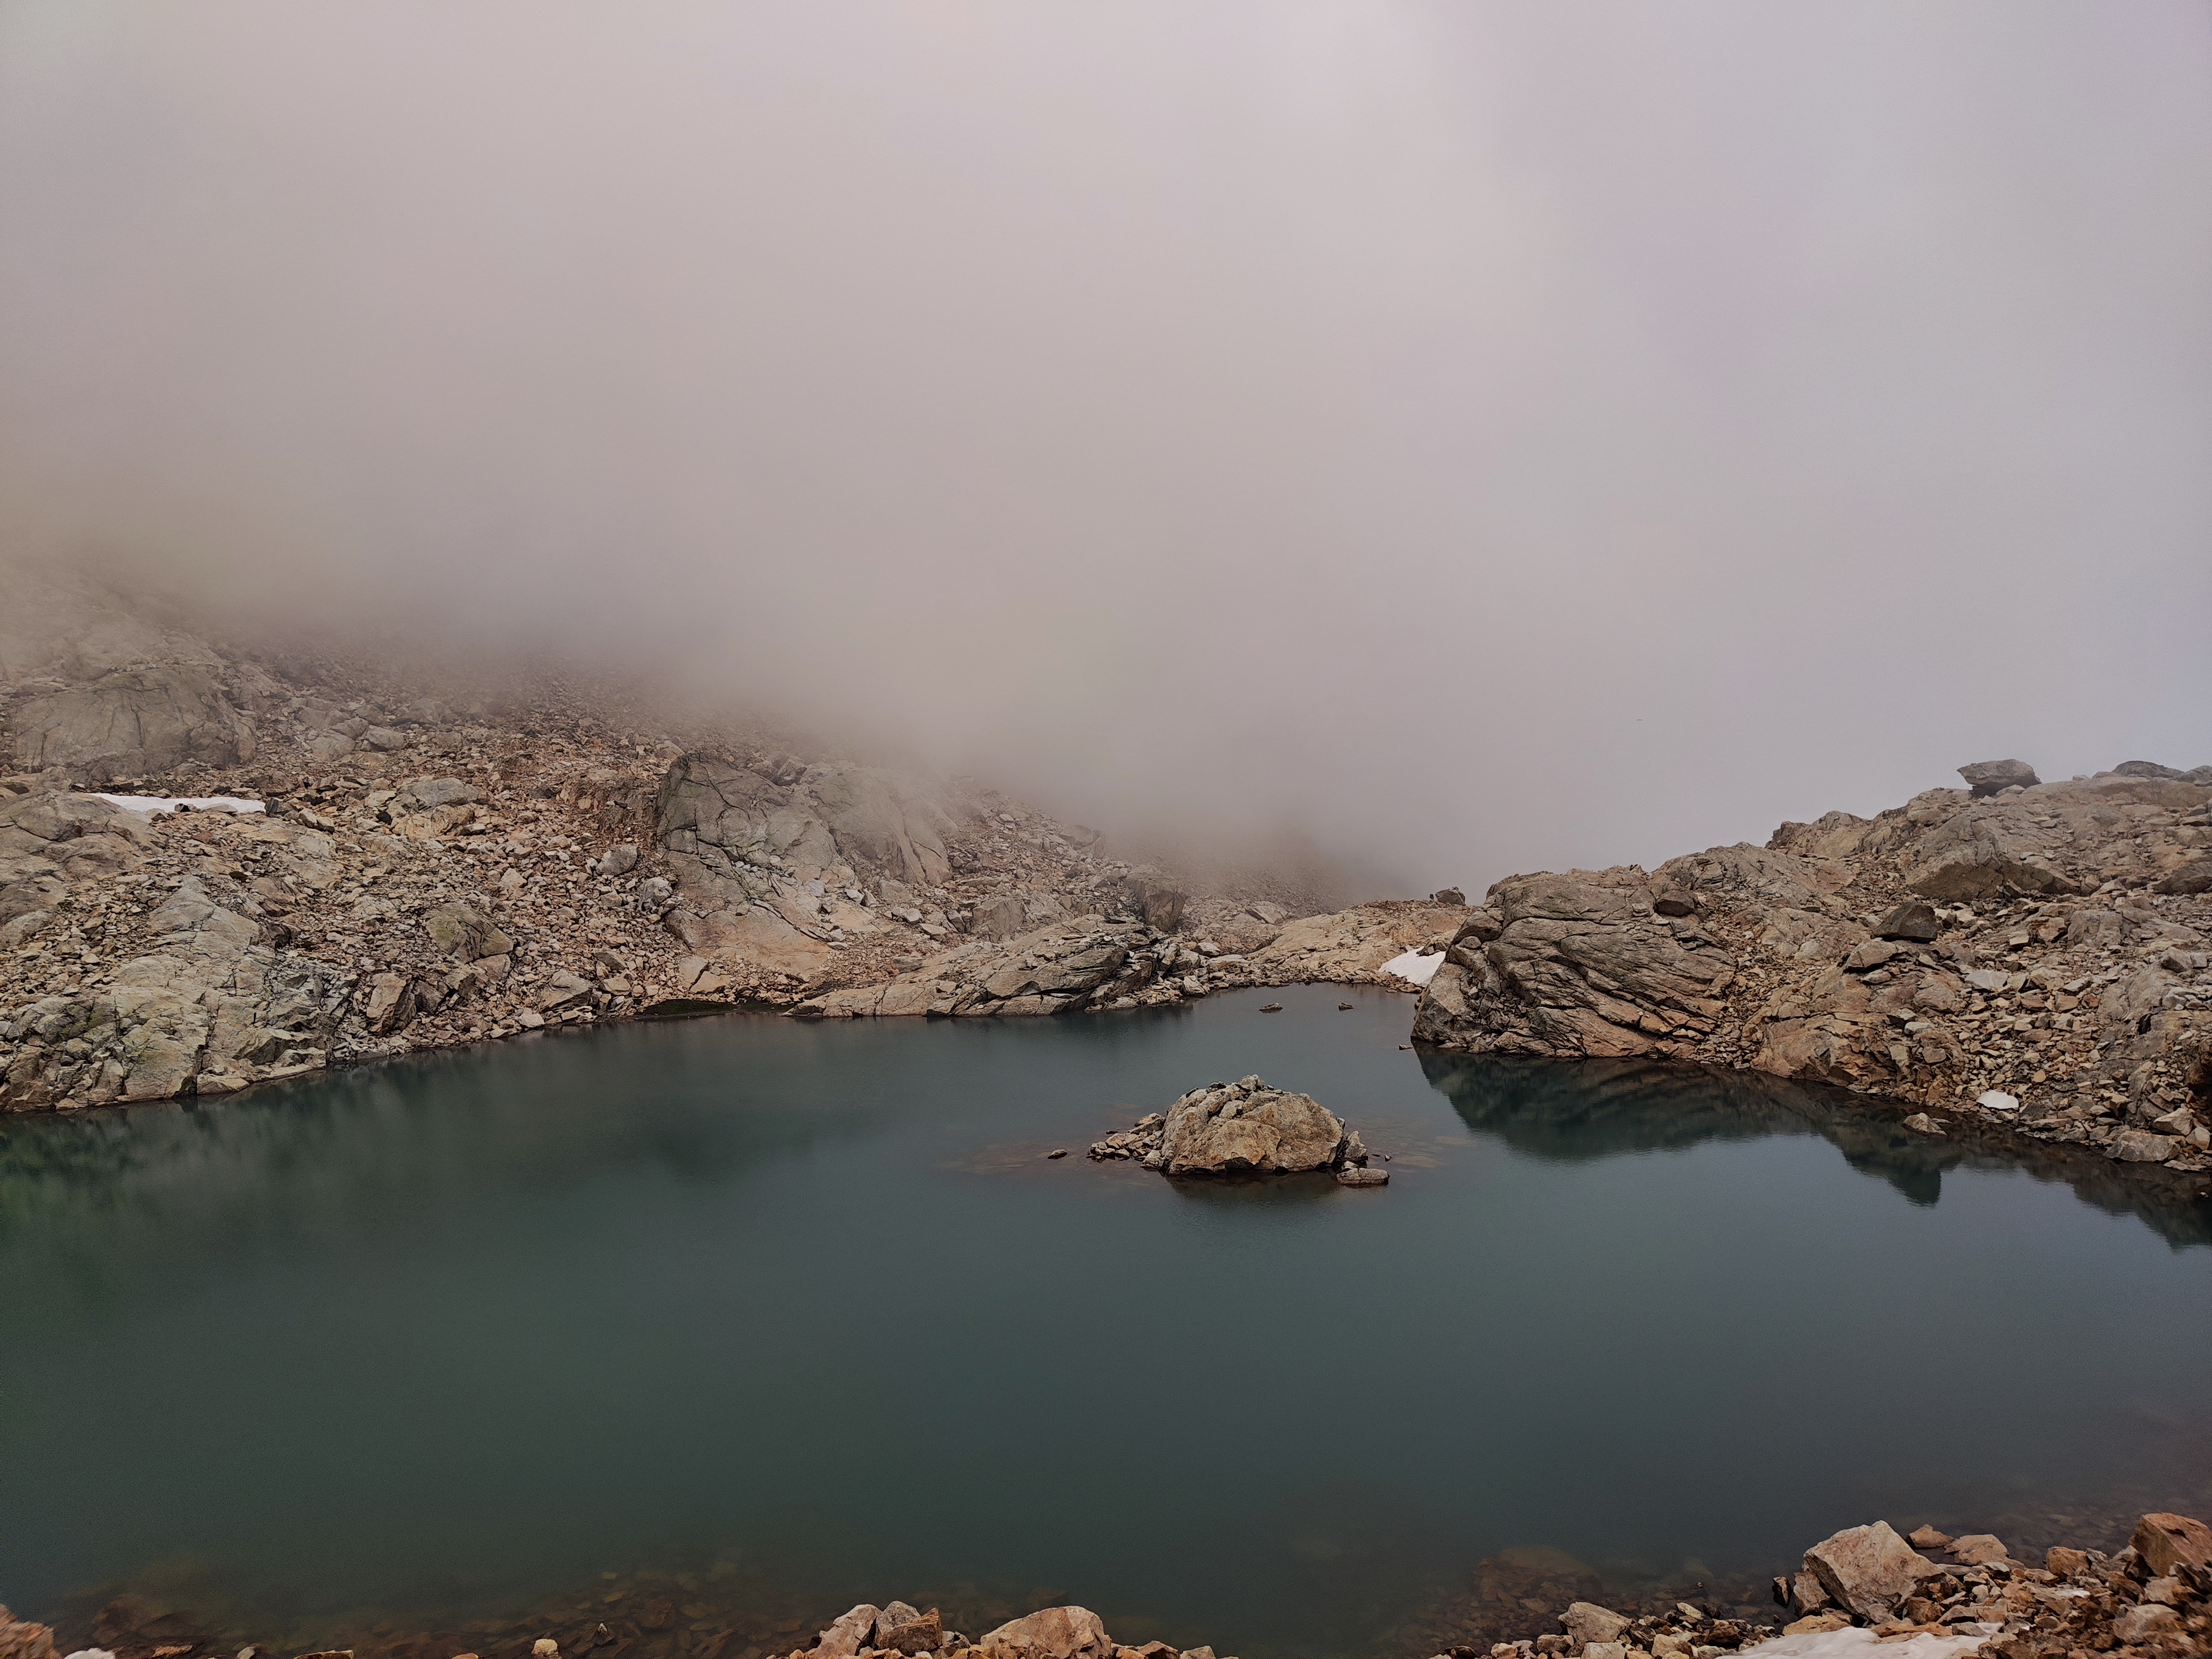
\includegraphics[angle=0, width=0.7\linewidth]{../pics/IMG_20240823_170306}
	\caption{Туман на озере под пер. Джалпаккол Северный}
	\label{fig:IMG_20240823_170306}
\end{figure} 

Дальнейший спуск отнял очень много сил, т.~к. из-за тумана шли практически полностью <<по приборам>> --- т.е. по навигатору --- с локальным ориентированием на местности в пределах 10--20~м. Спуск продолжал идти полностью по осыпи среднего и крупного размера; при этом на тропу либо так и не удалось выйти, либо она была крайне слабо читаемой. Добавляло сложности и то, что у Наташи болели колени, проблемы с которыми в условиях спуска по мокрым камням усугубились. 

С осыпи сошли в 18:10 , за 3 ходки с седловины перевала, довольно точно выйдя на тропу в зоне альпийского луга. Эта тропа идёт серпантином по склону, два раза обходя участки бараньих лбов. В условиях тумана и моросящего дождя спуск был довольно изматывающим физически и сильно изматывающим психологически. В зоне вторых бараньих лбов есть риск спустить камень на идущих ниже, поскольку тропа на этом участке идёт вниз практически не петляя. Этот этап занял 20 мин ЧХВ.

В 18:30 дошли до оборудованных стоянок на выполаживании травянисто-осыпного склона. (рис.~\ref{fig:IMG_20240823_184041}). Координаты м.н.: N~43.274531\degree, E~42.122488\degree.

\begin{figure}[h!]	
	\centering
	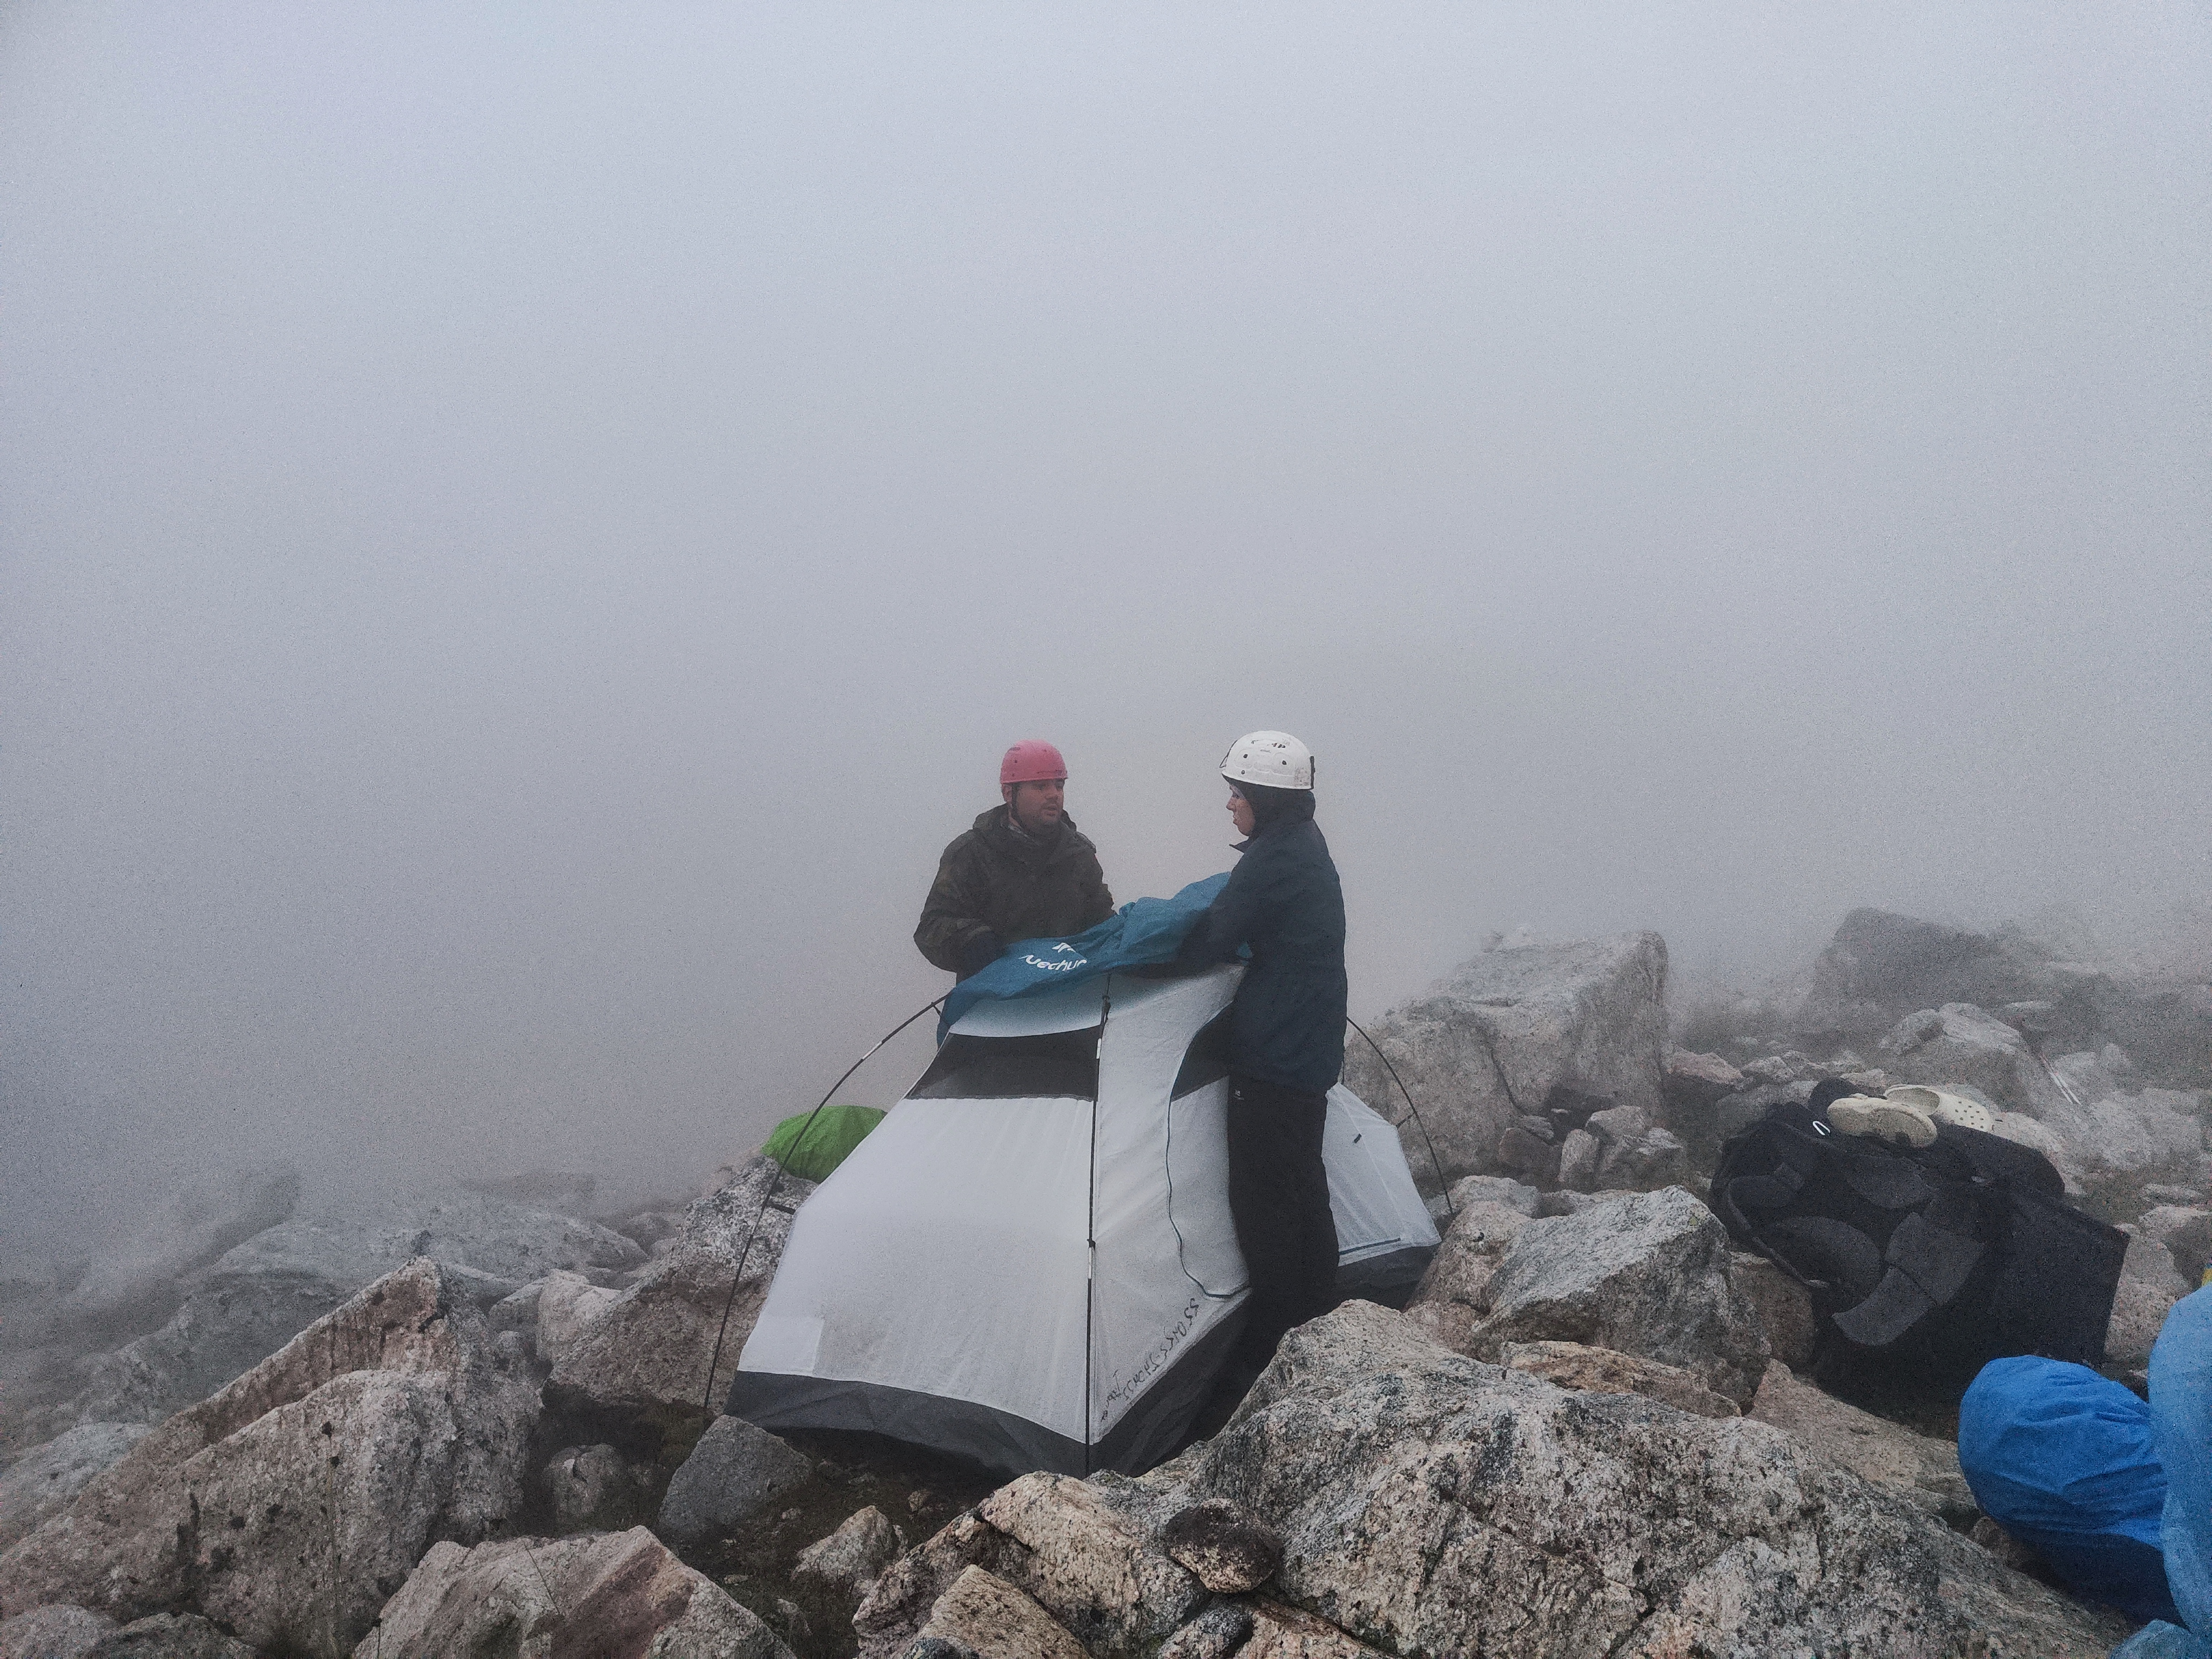
\includegraphics[angle=0, width=0.7\linewidth]{../pics/IMG_20240823_184041}
	\caption{м.н. 23-24 августа}
	\label{fig:IMG_20240823_184041}
\end{figure}

Высота ночёвки в этот день была максимальной за весь поход и составила 3050~м. Неприятным сюрпизом стало то, что источника воды в непосредственной близости от стоянок не оказалось, так как озеро у площадок пересохло. Ближайший источник воды нашёлся в 200~м к западу от м.н., в также почти пересохшем озере, которое спряталось за локальной возвышенностью (<<пупырь>>) около 100~м в диаметре. Относительно этой возвышенности озеро находилось на диаметрально противоположном конце от стоянки. Руководитель сходил на разведку, не дойдя до озера, но услышав воду, --- и по результатам этой разведки стало ясно, что в условиях такого тумана выходить за водой в одиночку крайне опасно. Ситуация была близкой к тому, чтобы не набирать воду вообще, однако в итоге решили выйти половиной группы --- включая руководителя и замруководителя,~--- чтобы в крайнем случае выстроиться в цепочку от озера до лагеря и быть в пределах видимости друг друга. Водоносы взяли с собой навигатор; оставшимся в лагере были выданы инструкции: при любом раскладе оставаться на месте и по истечении контрольного времени подавать голосовые команды. К нашему везению, в момент выхода водоносов из лагеря выдалось погодное окно, во время которого удалось дойти до озера всей группой, не выстраиваясь в цепочку. Пупырь обходили против часовой стрелки по крупной осыпи. 

Пока набирали воду, туман снова стал сгущаться. Путь в обратную сторону по курумнику был не самым приятным, и руководитель по виду рельефа предположил, что с другой стороны есть шансы выйти на травянистый участок, --- а также понадеялся, что тропа, уходящая от м.н. вниз, проходит где-то вблизи пупыря, --- поэтому группа водоносов продолжила обходить пупырь против часовой стрелки. Надежды подсечь тропу оказались ошибочными, а вот рельеф склона действительно сменился на травянистый --- но сам склон стал круче.\alert{(Возможно, я ещё услышала Катины крики именно с этой стороны --- надо уточнить у ребят.)} 

\alert{(Если это не так, то...)} Траверсирование склона в тумане в сумерках, практически полностью <<по приборам>> было достаточно стрессовым занятием. К огромному облегчению, когда до лагеря оставалась треть или четверть круга в обход пупыря, водоносы ясно услышали крики оставшихся в лагере, и, в частности, благодаря им, успешно нащупали дорогу к стоянке. Воду доставили в лагерь, и группа смогла приготовить горячий ужин. Весь выход за водой занял около 40 мин.

\begin{figure}[h!]	
	\centering
	\includegraphics[angle=0, width=0.7\linewidth]{../pics/IMG_20240823_205116}
	\caption{Звёздное небо}
	\label{fig:IMG_20240823_205116}
\end{figure}
 
Примерно в 21:00 туман рассеялся, и нам открылся потрясающий вид на Млечный путь (рис.~\ref{fig:IMG_20240823_205116}).
 
 \begin{table}[h!]
 	\centering
 	\begin{tabular}{|c|c|c|c|c|c|} 
 		\hline 
 		Этап & ЧХВ \\ 	
 		\hline 
 		От т/б <<Глобус>> до начала подъёма в д.р. Джалпаккол  & 00:44 \\
 		Подъём в д.р. Джалпаккол  & 02:33 \\
 		Подъём по д.р. Джалпаккол & 01:17\\ 
 		Подъём в д.р. Кичкинекол Джалпаккольский до подножия моренных валов & 02:08\\ 
 		По моренным валам до перевального взлёта & 03:42\\ 
 		По леднику & 00:28 \\
 		По скалам на седловину & 00:45 \\
 		Спуск к озеру & 00:40 \\
 		Спуск к ночёвкам на 3000 м & 01:51 \\
 		Спуск в д.р. Мырды & 02:08 \\
 		По д.р. Мырды до а/л <<Узункол>>& 01:45 \\
 		\hline
 		\textsc{Полное время подъёма на перевал  }& 10:37\\
 		\textsc{Полное время спуска с перевала }& 06:24 \\
 		\textsc{	Полное время прохождения перевала }& 17:01 \\
 		\hline
 	\end{tabular}
 	\caption{Расклад времени, пер. Джалпаккол Северный}
 \end{table}
 
 \paragraph{Выводы и рекомендации:} пер. Джалпаккол Северный соответствует заявленной категории трудности, разнообразен с точки зрения рельефа, однако может быть утомителен морально при движении по моренным валам. Перевал является хоршей обзорной точкой района, что с лихвой оправдывает утомительность подъёма. Перевал рекомендуется к прохождению в новичковых походах; впрочем, вероятно, не стоит ставить его первым на маршруте, если есть сомнения в физической и моральной подготовке группы.
 
\clearpage

\subsection{24 августа. А/л <<Узункол>>}
\textit{Метеоусловия: утром пасмурно, днём дождь, вечером переменная облачность.}

Подъём в 08:00, выход в 10:20. Сегодняшняя наша цель~--- спуститься в а/л <<Узункол>> и устроить там полуднёвку.


\begin{figure}[h!]
	\centering
	\includegraphics[width=0.7\linewidth]{../pics/DSC_0107.jpg}
	\caption{Верховья р. Мырды}
	\label{fig:DSC_0107.jpg}
\end{figure}


\newpage
\subsection{25 августа. Д.р. Кичкинекол}
\textit{Метеоусловия: утром, днём тепло, переменная обласность; после 17:00 дождь с грозой}

\begin{figure}[h!]
	\centering
	\includegraphics[angle=0, width=0.7\linewidth]{../pics/mini_maps/25}
	\label{fig:mini_25}
\end{figure}

Подъём в 6:30. Облачно, без осадков. Перепаковываемся (рис.~\ref{fig:DSC_0126.JPG}), оставляем некоторые вещи и продукты сходившему участнику группы (Наташе). 

\begin{figure}[h!]
	\centering
	\includegraphics[width=0.7\linewidth]{../pics/DSC_0126.JPG}
	\caption{Утренние сборы в а/л <<Узункол>>}
	\label{fig:DSC_0126.JPG}
\end{figure}

Выходим в 9:58 по левому берегу р. Узункол. В 10:45 оказываемся в ущелье р. Кичкинекол (рис.~\ref{fig:DSC_0127.JPG}). 

\begin{figure}[h!]
	\centering
	\includegraphics[width=0.7\linewidth]{../pics/DSC_0127.jpg}
	\caption{группа в ущелье р. Кичкинекол}
	\label{fig:DSC_0127.JPG}
\end{figure}


Грунтовка укатанная, регулярно проезжают машины.  В 11:12 проходим поворот на пер. Доломиты Южные (1А). Боясь пропустить поворот на косогор, ведущий к нашему перевалу Кичкинекол Малый, забираемся на склон, как оказывается позднее, за 200 м до начала тропы, и в 11:50 подсекаем хорошо набирую тропу (рис~\ref{fig:IMG_20240825_134744.jpg}).  
	
	\begin{figure}[h!]
		\centering
		\includegraphics[width=0.7\linewidth]{../pics/DSC_0138.jpg}
		\caption{Начало подъёма на косогор в д.р. Таллычат}
		\label{fig:DSC_0138.JPG}
	\end{figure}
	
	Возле водопада, на высоте 2365~м, в 13:06 делаем привал, чтобы набрать воды и поискать потерянные на переходе блокнот и бинокль (к сожалению, безуспешно). Далее по тропе набираем высоту по графику 15/10 минут. Погода была всё ещё пасмурной, но ничего движению не мешало. Мест для обеда не было, поэтому питались заначкой и сух.пайком.

\begin{figure}[h!]
	\centering
	\includegraphics[width=0.7\linewidth]{../pics/IMG_20240825_134744.jpg}
	\caption{Тропа по склону р. Кичкинекол к Таллычатским ночёвкам}
	\label{fig:IMG_20240825_134744.jpg}
\end{figure}


В 14:40 выходим из зоны леса к нижним Таллычатским ночёвкам. Нашему взору представляются потрясающие виды на ГКХ (рис.~\ref{fig:DSC_0158.JPG}). 

\begin{figure}[h!]
	\centering
	\includegraphics[width=0.7\linewidth]{../pics/DSC_0158.jpg}
	\caption{Вершины и перевалы ГКХ в районе пер. Кичкинекол}
	\label{fig:DSC_0158.JPG}
\end{figure}

Дальшейший путь до м.н. не представляет особого труда, если не учитывать красивые виды вокруг и обилие костяники под ногами.

В 16:04 приходим на наше м.н., пересохшее озеро, называющееся сейчас Поляной Крокусов. Ставим палатки, готовим ужин, и сразу после этого начинается сильный дождь. Непогода не прекращалась до часу ночи, некоторые участники были вынуждены рыть дренажные канавы, чтобы не затапливало палатки. Утром мы порадовались, что встали в верхней части стоянок, так как нижняя часть озера за ночь перестала быть пересохшей.
Координаты м.н. N43.249638\degree, E42.198292\degree.

\begin{figure}[h!]
	\centering
	\includegraphics[width=0.7\linewidth]{../pics/DSC_0177.jpg}
	\caption{м.н. 25-26 августа}
	\label{fig:DSC_0177.JPG}
\end{figure}




\newpage
\subsection{26 августа. Пер. Кичкинекол Малый}
\newpage
\subsection{27 августа. Пер. Перемётный (1А)}
\textit{Метеоусловия: утром, днём, вечером ясно, тепло.}

\begin{figure}[h!]
	\centering
	\includegraphics[angle=0, width=0.7\linewidth]{../pics/mini_maps/27}
	\label{fig:mini_27}
\end{figure}




\begin{figure}[h!]
	\centering
	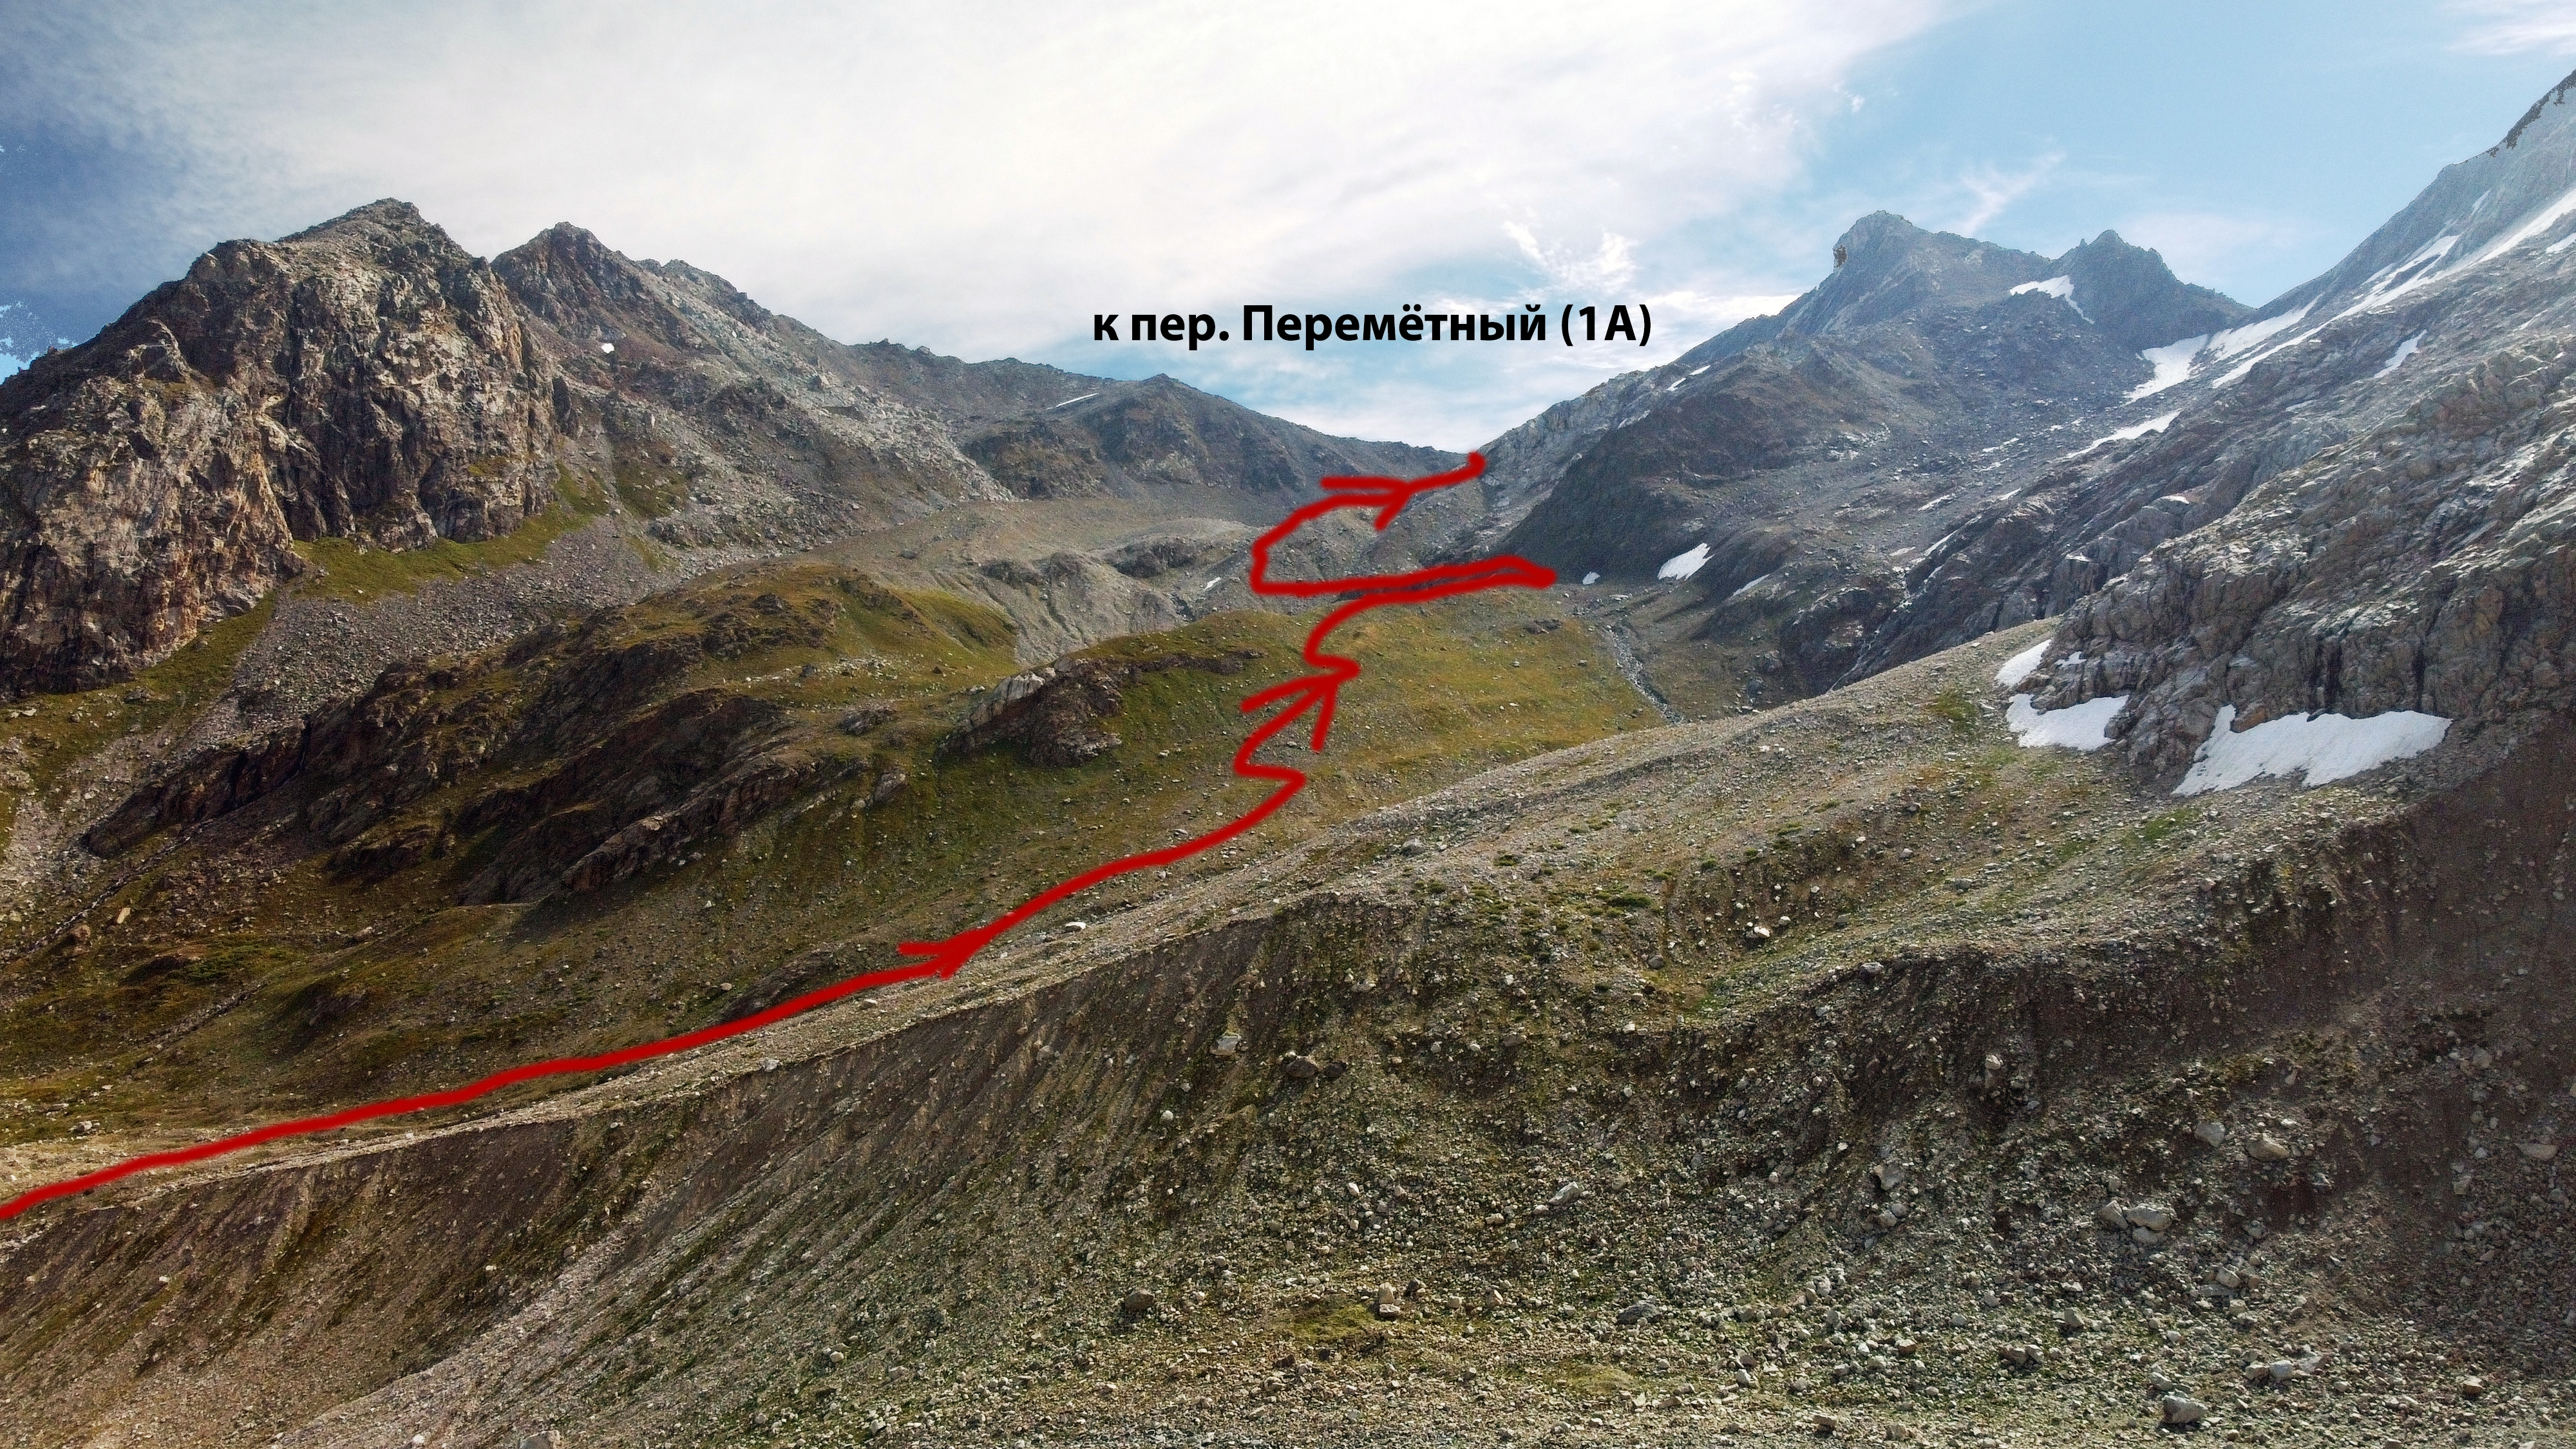
\includegraphics[width=0.7\linewidth]{../pics/perem_1}
	\caption{Начало подъёма к пер. Перемётный из д.р. Чунгур-Джар}
	\label{fig:perem_1}
\end{figure} 


Метеоусловия: солнечно, тепло

Утром проснулись в 7:00, долго стирались, чинились и сушились, руковод курил какао и размышлял... Переметный было решено брать!
В 10:00 выдвинуль в сторону перевала.

\begin{figure}[h!]
	\centering
	\includegraphics[width=0.7\linewidth]{../pics/DSC_0251.jpg}
	\caption{Утренний лагер. Активно сушимся.}
	\label{fig:DSC_0251}
\end{figure}

\textbf{Задача номер раз:} перейти многорукавье реки Чунгур-Джар. Оказалось сложнее, чем казалось. Часть группы промочила ботинки и усердно их сушила на каждом привале.

\begin{figure}[h!]
	\centering
	\includegraphics[width=0.7\linewidth]{../pics/DSC_0254.jpg}
	\caption{р. Чунгур-Джар. Нам предстоит перебраться через множество ручейков.}
	\label{fig:DSC_0254}
\end{figure}
\begin{figure}[h!]
	\centering
	\includegraphics[width=0.7\linewidth]{../pics/DSC_0277.jpg}
	\caption{р. Чунгур-Джар. Перебрались.}
	\label{fig:DSC_0277}
\end{figure}

\textbf{Задача номер два:} пройти подъем на перевал. Поднялись на морену по травянисто-каменстому склону, прошли по гребню и попрощались на время с травой. На высоте 2410м (N 43.24135, E 42.24827) начали траверс по сыпухе и под небольшой скалой на соседнюю морену.
\begin{figure}[h!]
	\centering
	\includegraphics[width=0.7\linewidth]{../pics/DSC_0280.jpg}
	\caption{Траверс по моренам.}
	\label{fig:DSC_0280}
\end{figure} 
После этого - прямым курсом на перевал. С задачей два справились в 14:38. На перевале сняли записку группы туристов из Ростова-на-Дону и Новочеркасска от 20.08.2019 \ref{pic:peremetnyy}. Примечательно, что эта группа в свое время сняла записку Горной секции МФТИ под руководством Королева Андрея от 2018 года - в этот поход ходила руковод.

\begin{figure}[h!]
	\centering
	\includegraphics[width=0.7\linewidth]{../pics/DSC_0419 2.jpg}
	\caption{Перевал Переметный. Вид на Эльбрус.}
	\label{fig:DSC_0419 2}
\end{figure} 

\textbf{Задача три:} спуститься в низ, в д.р. Танышхан. Здесь начинается очень интересная и поучительная история.
\begin{figure}[h!]
	\centering
	\includegraphics[width=0.7\linewidth]{../pics/perem_down.png}
	\caption{Спуск с перевала переметный.}
	\label{perem_down}
\end{figure} 
Выдвинулись в 15:38. Вниз сначала шли по сыпухе забирая влево, усердно считали моренные валы чтобы не ошибиться и не угодить в березняк. По пути старались расставлять турики, но время подгоняло, в маршруте мы были не  уверены и на полпути мы это дело забросили.  Потом начался травянистый склон, альпеншток альпеншточил на все 100. После спуска на 130 м выбрались на курумник, на котором не обошлось без легкого кровопролития. К сумеркам снова вышли на травянистый склон. Русло пересохшего ручья (N 43.25779° E 42.27107°), засыпанного крупными камнями, предоставило удобный вариант до спуска. К моменту, когда мы добрались до зарослей рододендронов, уже порядком стемнело (19:05), дальше по лощине шли с фонарикам. 

В 20:00 вышли на отличную стоянку на берегу реки Танышхан (N 43.26002, E 42.27489). Поужинали, и легли спать. С задачей три справились!


\clearpage
\subsection{28 августа. Д.р. Чиринкол}
Просто текст
\newpage
\subsection{29 августа. Д.р. Кубань}

\begin{figure}[h!]
	\centering
	\includegraphics[angle=0, width=0.3\linewidth]{../pics/mini_maps/29}
	\label{fig:mini_29}
\end{figure}

\newpage
\subsection{30 августа. Пер. Хотютау (1А)}
\textit{Метеоусловия: утром, днём солнечно, тепло, безветренно. После 15:00 туман, переменная облачность. Вечером дождь, гроза.}

\begin{figure}[h!]
	\centering
	\includegraphics[angle=0, width=0.7\linewidth]{../pics/mini_maps/30}
	\label{fig:mini_30}
\end{figure}




\begin{figure}[h!]
	\centering
	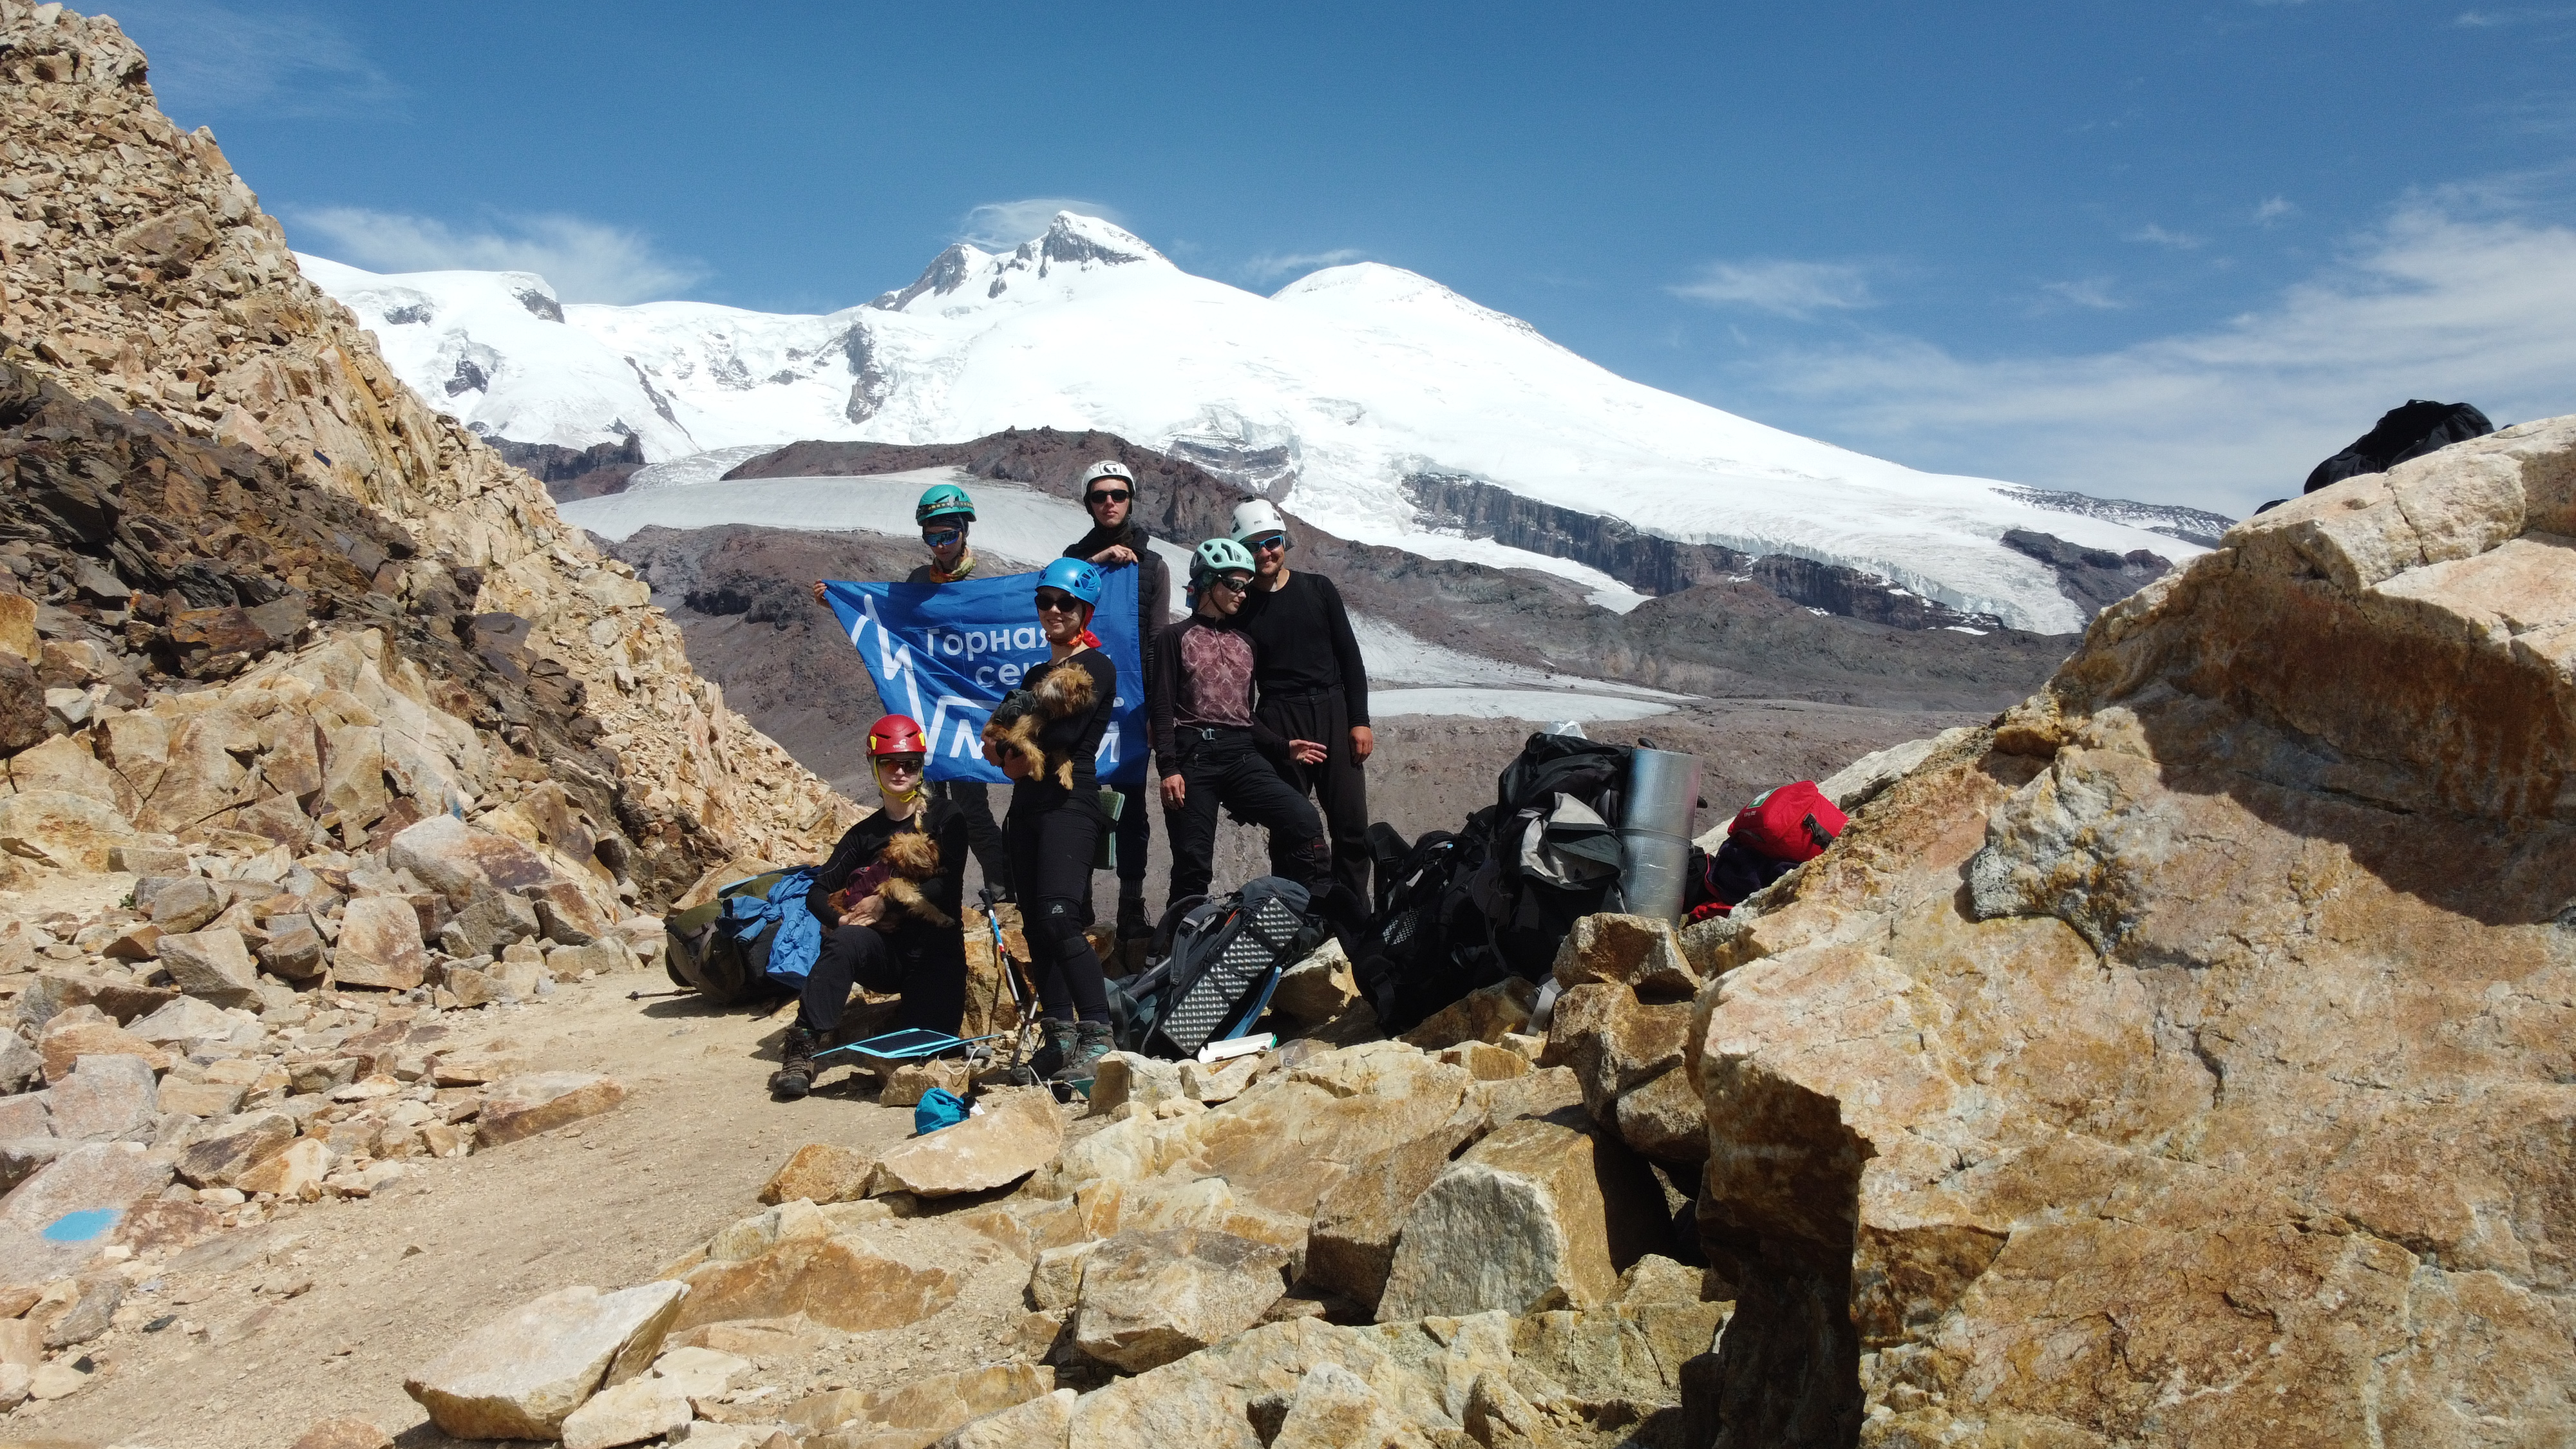
\includegraphics[width=0.7\linewidth]{../pics/DJI_0899}
	\caption{группа на пер. Хотютау}
	\label{fig:hotyutau_1}
\end{figure}

Мы проснулись утром рано на этой исхоженной площадочке. Позавтракали двойной порцией сухого омлета и отправились в путь.
До перевала ползли без особых проблем - сыпуха и курумник к концу похода стали нам родными и знакомыми. Огромной поддержкой оказались синие метки трека для трейл-раннеров. Они значительно сократили нам время на поиск пути.

В .. взошли на перевал. Полюбовались Эльбрусом, обломками вертолета на его склоне и букетом памятных табличек на самом перевале. Сняли записку проекта "Виртуальные горы" от 28.08.2024 и турклуба "ЛИИЖТ" г. Санкт - Петербург от 21.08.2024.

В .. начали спуск с перевала. Спуск по песчаному склону неприятный, но быстрый. В .. (N, E) надели кошки, подвязались блокировкой и начали движение по леднику. Ледник был открытый, трещины хорошо просматривались и легко обходились.

*Вставить фотографию собачек в ботиночках*

Через несколько минут нас нагнала группа из двху человек из горной секции МАИ. Как выяснилось, оставленная нами записка пролежала в камнях не более получаса :) Увеличенным составом мы двигаемся по леднику до начала ледопада, где подро сворачиваем налево и плутаем в обачном тумане, пока зоркий глаз не выцепляет вдалеке знокмую синюю метку. По портоптанной дорожке далее едем без проблем. 

В .. выходим к Эльбрусскому озеру. В этот момент выясняется, что до закрытия канатной дороги остается меньше получаса. Остаток пути идём на всех парах и садимся в кабинку в 17:00 ровно. Спустившись в поляну Азау, оплачиваем безбилетный проезд в закрытой , но приоткрывшейся специально для нас кассе. На этом мы прощаемся с нашими новыми друзьями и горная часть нашего путешествия завершается.

Хорошо проводим время в заведении "не помню". В 20:00 нас встречает микроавтобус и везет нас до вокзала "не помню" где мы встречаемся с частью слившихся участников. После полуночи загружаемся в поезд и катим домой!!!







\newpage
\section{Материальное обеспечение группы}

\begin{table}[h!]
	\centering
%	\resizebox{0.77\textwidth}{!}{%
		\begin{tabular}{|>{\centering\arraybackslash}m{0.02\linewidth}|>{\centering\arraybackslash}m{0.31\linewidth}|>{\centering\arraybackslash}m{0.08\linewidth}|>{\centering\arraybackslash}m{0.29\linewidth}|>{\centering\arraybackslash}m{0.08\linewidth}|}
			\hline
			\multirow{2}{*}{\textnumero}	&	\multicolumn{2}{|c|}{Личное}	&	\multicolumn{2}{|c|}{Специальное}	\\
			
			\cline{2-5} & Наименование	&	Кол-во	&	Наименование	&	Кол-во\\
			\hline
			1	&	Верёвка статическая 50~м, $\varnothing=9$~мм	&	1	&	Система с блокировкой	&	1	\\
			\hline
			2	&	Общественные карабины	&	5	&	Карабины	&	3	\\
			\hline
			3	&	Ледобуры	&	2	&	Спусковое устройство	&	1	\\
			\hline
			4	&	Станционные петли 180~см	&	3	&	Жумар	&	1	\\
			\hline
			5	&	Общественный корделет	&	2	&	Прусик короткий	&	2	\\
			\hline
			6	&	GPS-навигатор	&	1	&	Ледоруб	&	1	\\
			\hline
			7	&	Спутниковый треккер	&	1	&	Каска	&	1\\
			\hline
			8	&	&		&	Кошки	&	1 пара\\
			\hline
			9	&	&		&	Солнцезащитные очки	&	1\\
			\hline

		\end{tabular}%
%	}
\end{table}



\newpage
\section{Стоимость снаряжения, питания, проживания, транспортныые расходы}

Тут будет табличка от Ильи

\newpage
\section{Итоги похода, выводы и рекомендации по совершенному походу}
\newpage
\section{Использованные материалы, карты и фотографии}
\newpage

\section{Перевальные записки}

\begin{figure}[h!]
	\begin{minipage}[h!]{0.49\linewidth}
		\centering{\includegraphics[width=0.98\linewidth]{../pics/notes/ullukuel_front}}
	\end{minipage}
	\hfill
	\begin{minipage}[h!]{0.49\linewidth}
		\centering{\includegraphics[width=0.98\linewidth]{../pics/notes/ullukuel_rev}}
	\end{minipage}
	\caption{Записка с пер. Уллу-Кёль Восточный}
	\label{pic:ullu_kuel}
\end{figure}

\begin{figure}[h!]
	\begin{minipage}[h!]{0.325\linewidth}
		\centering{\includegraphics[width=0.98\linewidth]{../pics/notes/dzhalpakkol1_front}}
	\end{minipage}
	\hfill
	\begin{minipage}[h!]{0.325\linewidth}
		\centering{\includegraphics[width=0.98\linewidth]{../pics/notes/dzhalpakkol1_rev}}
	\end{minipage}
	\hfill
	\begin{minipage}[h!]{0.325\linewidth}
		\centering{\includegraphics[width=0.98\linewidth]{../pics/notes/dzhalpakkol2_front}}
	\end{minipage}
	\caption{Записки с пер. Джалпаккол Северный}
	\label{pic:dzhalpakkol}
\end{figure}

\begin{figure}[h!]
	\begin{minipage}[h!]{0.49\linewidth}
		\centering{\includegraphics[width=0.7\linewidth]{../pics/notes/kichkinekol_front}}
	\end{minipage}
	\hfill
	\begin{minipage}[h!]{0.49\linewidth}
		\centering{\includegraphics[width=0.7\linewidth]{../pics/notes/kichkinekol_rev}}
	\end{minipage}
	\caption{Записка с пер. Кичкинекол Малый}
	\label{pic:kichkinekol}
\end{figure}

\begin{figure}[h!]]
	\centering{\includegraphics[width=0.7\linewidth]{../pics/notes/peremetnyy_front}}
	\caption{Записка с пер. Перемётный}
	\label{pic:peremetnyy}
\end{figure}

\begin{figure}[h!]
	\begin{minipage}[h!]{0.325\linewidth}
		\centering{\includegraphics[width=0.98\linewidth]{../pics/notes/hotyutau1_front}}
	\end{minipage}
	\hfill
	\begin{minipage}[h!]{0.325\linewidth}
		\centering{\includegraphics[width=0.98\linewidth]{../pics/notes/hotyutau2_front}}
	\end{minipage}
	\hfill
	\begin{minipage}[h!]{0.325\linewidth}
		\centering{\includegraphics[width=0.98\linewidth]{../pics/notes/hotyutau2_rev}}
	\end{minipage}
	\caption{Записки с пер. Хотютау}
	\label{pic:hotyutau}
\end{figure}
\clearpage



%\bibliography{Gvandra2024_biblio.bib}
\printbibliography



\end{document}